%% LyX 1.3 created this file.  For more info, see http://www.lyx.org/.
%% Do not edit unless you really know what you are doing.
\documentclass[english, 12pt]{article}
\usepackage{times}
%\usepackage{algorithm2e}
\usepackage{url}
\usepackage{bbm}
\usepackage[T1]{fontenc}
\usepackage[latin1]{inputenc}
\usepackage{geometry}
\geometry{verbose,letterpaper,tmargin=2.5cm,bmargin=2.5cm,lmargin=2.5cm,rmargin=2.5cm}
\usepackage{rotating}
\usepackage{color}
\usepackage{graphicx}
\usepackage{amsmath, amsthm, amssymb}
\usepackage{setspace}
\usepackage{lineno}
\usepackage{hyperref}
\usepackage{bbm}


\linenumbers
\doublespacing
%\usepackage[authoryear]{natbib}
\usepackage{natbib} \bibpunct{(}{)}{;}{author-year}{}{,} 

%Pour les rajouts
\usepackage{color}
\definecolor{trustcolor}{rgb}{0,0,1}

\usepackage{dsfont}
\usepackage[warn]{textcomp}
\usepackage{adjustbox}
\usepackage{multirow}
\usepackage{graphicx}
\graphicspath{{../figures/}}
\DeclareMathOperator*{\argmin}{\arg\!\min}

\let\tabbeg\tabular
\let\tabend\endtabular
\renewenvironment{tabular}{\begin{adjustbox}{max width=\textwidth}\tabbeg}{\tabend\end{adjustbox}}

\makeatletter

%%%%%%%%%%%%%%%%%%%%%%%%%%%%%% LyX specific LaTeX commands.
%% Bold symbol macro for standard LaTeX users
%\newcommand{\boldsymbol}[1]{\mbox{\boldmath $#1$}}

%% Because html converters don't know tabularnewline
\providecommand{\tabularnewline}{\\}

\usepackage{babel}
\makeatother


\begin{document}


\title{Joint estimation of SNP effects improves the prediction of complex diseases // Predicting complex diseases: performance and robustness [OF NEW METHOD?]}
\author{Florian Priv\'e\,$^{\text{ 1,}*}$, Hugues Aschard\,$^{\text{2}}$ and Michael G.B. Blum\,$^{\text{1,}*}$}



\date{~ }
\maketitle

\noindent$^{\text{\sf 1}}$Universit\'e Grenoble Alpes, CNRS, Laboratoire TIMC-IMAG, UMR 5525, France, \\
\noindent$^{\text{\sf 2}}$Centre de Bioinformatique, Biostatistique et Biologie Int\'egrative (C3BI), Institut Pasteur, Paris, France.

\noindent$^\ast$To whom correspondence should be addressed.

\newpage

\abstract{
Polygenic Risk Scores (PRSs) consist in combining the information across many single-nucleotide polymorphisms (SNPs) in a score reflecting the genetic risk of developing a disease. PRSs can have a major public health impact, allowing for screening campaigns to identify high-genetic risk individuals for a given disease.  The most commonly used method to derive PRSs is called ``Clumping+Thresholding'' (C+T). It uses only univariate genome-wide association studies (GWAS) summary statistics, which makes it very suitable and fast. However, PRS rely on non-optimal heuristics to account for correlation and to reduce noise in the predictor. 

In R package bigstatsr, we implemented a logistic regression model that provides a joint estimation of SNP effects. We used an efficient algorithm with new implementation tricks in order for this model to be used on huge datasets as large as the UK Biobank.

In this paper, we present a comprehensive comparative study of the C+T method, our penalized logistic regression and the T-Trees algorithm, which is a derivation of random forests. The penalized logistic regression consistently achieves higher predictive performance than the two other methods while being faster than the C+T method. 
Moreover, predictive performance of the C+T method is very sensitive to the threshold of inclusion of SNPs, whose optimal value depends on disease architecture. 
The improvement in predictive performance is more pronounced when there are few effects located in nearby genomic regions with correlated SNPs, or when sample size is increasing. 
When analyzing real SNP data from a case-control study,  penalized logistic regression provides an AUC of 89\% while the standard C+T method provides a smaller AUC of 82\%.

Instead of computing polygenic risk scores based on GWAS univariate summary statistics, we recommend to use penalized logistic regression as implemented in the R package bigstatsr to obtain more accurate polygenic risk scores when individual genotype data are available.\\

\textbf{Contact:} \href{florian.prive@univ-grenoble-alpes.fr}{florian.prive@univ-grenoble-alpes.fr} \& \href{michael.blum@univ-grenoble-alpes.fr}{michael.blum@univ-grenoble-alpes.fr}\\
\textbf{Supplementary information:}
}


%%%%%%%%%%%%%%%%%%%%%%%%%%%%%%%%%%%%%%%%%%%%%%%%%%%%%%%%%%%%%%%%%%%%%%%%%%%%%%%%

\newpage
\section{Introduction}

Polygenic Risk Scores (PRSs) consist in combining the information across many single-nucleotide polymorphisms (SNPs) in a score reflecting the genetic risk of developing a disease. PRSs are useful for different applications, such as testing polygenicity of a disease and finding a common genetic contribution between two diseases \cite[]{purcell2009common}. 
Personalized medicine is another major application of PRSs. Personalized medicine envisions to use PRSs in screening campaigns in order to identify high-risk individuals for a given disease \cite[]{chatterjee2016developing}. As an example of practical application, targeting screening to men at higher polygenic risk could reduce the problem of overdiagnosis and lead to a better benefit-to-harm balance in screening for prostate cancer \cite[]{pashayan2015implications}. 
Moreover, screening based on sequencing seems to make individuals positively change their health behavior, while neither causing patient anxiety nor depression \cite[]{vassy2017impact}.
Yet, PRSs would have to show a high discriminative power between cases and controls in order to be used for helping in the diagnosis of diseases. 
For example, for screening high-risk individuals and for presymptomatic diagnosis of the general population, it is suggested that the AUC must be greater than 75\% and 99\% respectively \cite[]{janssens2007impact}.

Many methods have been developed to predict disease status, or more generally any phenotype, based on SNP information.
A commonly used method, called ``P+T'' or ``C+T'' (which stands for ``Clumping and Thresholding'') -- or even just PRS -- is used to derive PRSs from results of Genome-Wide Association Studies (GWASs) \cite[]{chatterjee2013projecting,dudbridge2013power,evans2009harnessing,purcell2009common,wray2007prediction}. 
This technique uses GWAS summary statistics only, which makes it very convenient to compute and also very fast.
Linear Mixed-Models (LMMs) are another widely-used method in fields such as plant and animal breeding or for predicting highly heritable quantitative human phenotypes such as height \cite[]{lello2017accurate,yang2010common}. 
Yet, the predictions resulting from LMM, known e.g.\ as ``gBLUP'', are not designed for binary traits such as a disease status and are not optimal in this setting \cite[]{abraham2013performance}. 
Moreover, these methods and their derivatives are often computationally demanding, both in terms of memory and time requirements, which makes them unlikely to be used for prediction on very large datasets \cite[]{golan2014effective,maier2015joint,speed2014multiblup,zhou2013polygenic}.
Finally, statistical learning methods have also been used to derive PRSs for complex human diseases by jointly estimating SNP effects. Such methods include logistic regression, Support Vector Machine (SVM) and random forests \cite[]{abraham2012sparsnp,abraham2014accurate,botta2014exploiting,okser2014regularized,wei2009disease}.

We recently developed two R packages, bigstatsr and bigsnpr, for efficiently analyzing large-scale genome-wide data \cite[]{prive2017efficient}. Package bigstatsr includes an efficient algorithm with new implementation tricks for computing sparse linear and logistic regressions on huge datasets as large as the UK Biobank \cite[]{bycroft2017genome}.
In this paper, we present a comprehensive comparative study of the C+T method, our implementation of penalized logistic regression and the T-Trees algorithm, a derivation of random forests that has shown high predictive performance \cite[]{botta2014exploiting}. 
Note that in this comparison we do not include any LMM method for the reasons mentioned before and do not include any SVM method because it is expected to give similar results to logistic regression \cite[]{abraham2012sparsnp} [<- IN METHODS? MAIS BIEN AUSSI DE DIRE PQ TOT..].
For the C+T model, we compare different thresholds of inclusion of SNPs.
For the logistic regression, we include two novel approaches. 
First, we introduce a procedure that we call Cross-Model Selection and Averaging (CMSA) for automatically choosing the regularization parameter of the penalized logistic regression, which directly affects the number of SNPs included in the model. 
We also show how to use feature engineering in order to capture not only linear effects, but also recessive and dominant effects.

There have already been comparative studies on predicting human binary phenotypes based on genotype data. 
\cite{abraham2013performance} showed that sparse penalized methods performed better than the standard C+T method and LMMs, for a wide-range of human diseases.
\cite{zhou2013polygenic} used simulations on real genotypes of Australian individuals to show that a hybrid of linear mixed models and sparse regression models performed better in a range of sparse to polygenic disease architectures. 
\cite{spiliopoulou2015genomic} investigated the effect of relatedness in prediction performance.
\cite{ware2017heterogeneity} evaluated best practices for using the C+T method and found out that the optimal inclusion threshold is trait-dependent. 
In this study, we particularly extend the work of \cite{abraham2013performance} by using a simulation framework similar but more extenstive than the one used in \cite{zhou2013polygenic}. 
In order to make our comparison as comprehensive as possible, we compare different disease architectures by varying the number, size and location of causal effects as well as the heritability. We also compare different models for generating liability scores, one with only linear effects, and one which combines linear, dominant and interaction-type effects.

First, we quickly discard T-Trees because this method shows lower predictive performance as compared to other methods, while being computationally demanding.
Then, we show that the penalized logistic regression consistently achieves higher predictive performance while being faster than the C+T method, whereas predictive performance of the C+T method is very sensitive to the threshold of inclusion of SNPs, depending on the disease architecture, as shown in \cite{ware2017heterogeneity}.



%%%%%%%%%%%%%%%%%%%%%%%%%%%%%%%%%%%%%%%%%%%%%%%%%%%%%%%%%%%%%%%%%%%%%%%%%%%%%%%%

\section{Methods}

\subsection{Genotype data}

We use real genotypes of European individuals from a case-control celiac disease study \cite[]{dubois2010multiple}. The composition of this dataset is presented in table \ref{tab:celiac-data}.
Details of quality control and imputation for this dataset are available in \cite{prive2017efficient}.
As for simulations presented here, in order to remove the genetic structure induced by the celiac disease status, we first restrict our simulations to controls. 
Then, we decided to remove population structure because it can affect the predictive performance of methods \cite[]{martin2017human}.
In order to alleviate population structure, we keep people from the UK only and we further remove outliers based on the robust Mahalanobis distances computed using the first 10 principal components of remaining individuals. 
This 3-step filtering process results in a sample of 7102 individuals with minimal population structure (see supplementary notebook ``preprocessing''). 

\subsection{Simulations of phenotypes} \label{sec:simus}

In order to simulate phenotypes, we use the Liability Threshold Model (LTM) with a prevalence of 30\% \cite[]{falconer1965inheritance}. We vary different parameters: the number of chromosomes used (either all 22 chromosomes or chromosome 6 only), the size of the training set (from 1000 to 6000), the number of causal variants and their location (30, 300 or 3000 anywhere on the genome or 30 only in the HLA region), the heritability (50\% or 80\%), the distribution of effects associated with causal SNPs (Normal or Laplace). We also use two different models to compute liability scores: a ``simple'' model with linear effects only, and a ``fancy'' model which combines linear, dominant and interaction-type effects.
For the ``simple'' model, we compute $$y_i = \sum_{j\in S_\text{causal}} w_j \cdot \widetilde{G_{i,j}}$$ where $w_j$ are weights generated with a Gaussian or a Laplace distribution, $G_{i,j}$ is the allele count of individual $i$ for SNP $j$ and $\widetilde{G_{i,j}}$ corresponds to its standardized version (zero mean and unit variance for all SNPs). 
For the ``fancy'' model, we separate the causal SNPs in three equal sets $S_\text{causal}^{(1)}$, $S_\text{causal}^{(2)}$ 
and $S_\text{causal}^{(3)}$; $S_\text{causal}^{(3)}$ is further separated in two equal sets, $S_\text{causal}^{(3.1)}$ and $S_\text{causal}^{(3.2)}$. 
We then compute $$y_i = \underbrace{\sum_{j\in S_\text{causal}^{(1)}} w_j \cdot \widetilde{G_{i,j}}}_\text{linear} + \underbrace{\sum_{j\in S_\text{causal}^{(2)}} w_j \cdot \widetilde{D_{i,j}}}_\text{dominant} + \underbrace{\sum_{\substack{k=1 \\ j_1=e_k^{(3.1)} \\ j_2=e_k^{(3.2)}}}^{k=\left|S_\text{causal}^{(3.1)}\right|} w_{j_1} \cdot \widetilde{G_{i,j_1} G_{i,j_2}}}_\text{interaction}$$ 
where $D_{i,j} = \mathds{1}\left\{G_{i,j} \neq 0\right\}$ and $S_\text{causal}^{(q)}=\left\{e_k^{(q)},~k \in \left\{1, \ldots, \left|S_\text{causal}^{(q)}\right|\right\}\right\}$. 
Note that for the interaction part of the model, we scale interactions, not the raw allele counts, so that corresponding SNPs still have a marginal effect. 
For both models, the values of $y_i$ are then standardized so that they have a variance equal to the desired heritability $h^2$ and we further add some environmental noise $\epsilon_i$ to $y_i$, where $\epsilon \sim N(0, 1 - h^2)$.


We implement 3 different simulation scenarios, summarized in table \ref{tab:simus}. 
Scenario \textnumero1 uses the whole dataset (all 22 autosomal chromosomes) and a training set of size 6000. 
It compares all methods described in section \ref{sec:methods}; for each combination of the remaining parameters, results are based on 100 simulations (i.e.\ 5 times more than in \cite{zhou2013polygenic}). 
However, comparison results for T-Trees relies on 5 simulations only (and an heritability of 80\%) because this method can require several hours of computation for a single simulation. 
Scenario \textnumero2 consists of 100 simulations per combination of parameters on a dataset composed of chromosome 6 only. Reducing the number of SNPs aims at increasing the polygenicity (the proportion of causal SNPs) of the simulated models and at virtually increasing the sample size \cite[]{dudbridge2013power,marquez2017multiethnic,vilhjalmsson2015modeling}. 
For this scenario, we use only the additive (``simple'') model, but continue to compare all previous different values of the other parameters.
Finally, scenario \textnumero3 reuses the whole dataset but this time varying the size of the training set in order to assess how the sample size affects predictive performance of methods. A total of 100 simulations per combination of parameters are run using 300 causal SNPs anywhere on the genome. 


\subsection{Predictive performance measures}\label{sec:auc}

In this study, we use two different measures of predictive accuracy. 
First, we use the Area Under the Receiver Operating Characteristic (ROC) Curve (AUC) \cite[]{fawcett2006introduction,hanley1982meaning,lusted1971signal}. In the case of our study, the AUC is the probability that a PRS of a case is greater than the PRS of a control.
This measure indicates the extent to which we can distinguish between cases and controls using PRSs.
As a second measure, the partial AUC for specificities between 90\% and 100\% is also reported \cite[]{dodd2003partial,mcclish1989analyzing}. This measure is similar to the AUC, but focuses on high specificities, which is the most useful part of the ROC curve in clinical settings. 

When reporting results of AUC, we use estimates of maximum achievable AUC values for the simulations: 84\% and 94\% for heritabilities of respectively 50\% and 80\% based on three different estimations (see Supplementary Materials). 

%Note that we also report the timing of the main computations and the number of SNPs used in the predictions.

\subsection{Methods compared} \label{sec:methods}

In this study, we compare three different types of methods: the C+T method, T-Trees and penalized logistic regression.

The C+T (Clumping + Thresholding) method directly derives a Polygenic Risk Score (PRS) from the results of a Genome-Wide Associations Study (GWAS), referred to as summary statistics.
In the GWAS, a coefficient of regression (estimated effect size) is learned independently for each SNP along with a corresponding p-value. 
The SNPs are first clumped (C) so that there remain only loci that are weakly correlated with one another, which form a set of SNPs denoted $S_\text{clumping}$. 
Then, thresholding (T) consists in removing SNPs with p-values larger than a threshold $p_T$ to be determined. 
Finally, a PRS is defined as the sum of allele counts of the remaining SNPs weighted by the corresponding effect coefficients: $$\rm{PRS}_i = \sum_{\substack{j \in S_\text{clumping} \\ p_j~<~p_T}} \hat\beta_j \cdot G_{i,j}$$ where $\hat\beta_j$ ($p_j$) are the effect sizes (p-values) learned from the GWAS. In this study, we report scores for a clumping threshold at $r^2 > 0.2$ within regions of 500kb. 

For the C+T method, we report three different scores of prediction: one including all the SNPs (remaining after clumping), one including only SNPs that have a p-value under the GWAS threshold of significance ($p < 5 \cdot 10^{-8}$), and one that maximizes the AUC for these two thresholds and a sequence of 100 values of thresholds ranging from $10^{-0.1}$ to $10^{-100}$ and equally spaced on the log-log-scale (Table \ref{tab:thr}). 
As we report the optimal threshold based on the test set, the corresponding AUC value is an upper bound of the AUC for the C+T method.
We call these three reported scores respectively ``PRS-all'', ``PRS-stringent'' and ``PRS-max'' in the results.

T-Trees (\textit{Trees inside Trees}) is an algorithm derived from random forests \cite[]{breiman2001random} that takes into account the correlation structure among the genetic markers implied by linkage disequilibrium in GWAS data \cite[]{botta2014exploiting}. We use the same parameters as reported in Table 4 of \cite{botta2014exploiting}, except that we use 100 trees instead of 1000 because because using 1000 trees provides a minimal increase of AUC while requiring a disproportionately long processing time (e.g.\ AUC of 81.5\% instead of 81\%, data not shown). %We call this method ``T-Trees'' in the results.

Finally, for the penalized logistic regression, we solve: $$\arg\!\min_{\beta_0,~\beta}(\lambda, \alpha)\left\{  \underbrace{ -\sum_{i=1}^n \left( y_i \log\left(p_i\right) + (1 - y_i) \log\left(1 - p_i\right) \right) }_\text{Loss function}   +   \underbrace{ \lambda \left((1-\alpha)\frac{1}{2}\|\beta\|_2^2 + \alpha \|\beta\|_1\right) }_\text{Penalization}  \right\}$$ where $p_i=1/\left(1+\exp\left(-(\beta_0 + x_i^T\beta)\right)\right)$, $x$ is denoting the genotypes and covariables (e.g.\ principal components), $y$ is the disease status we want to predict and $\lambda$ is a regularization parameter that needs to be determined. 
Different regularizations can be used to prevent overfitting, among other benefits: the L2-regularization (``ridge'', \cite{hoerl1970ridge}) shrinks coefficients and is ideal if there are many predictors drawn from a Gaussian distribution (corresponds to $\alpha = 0$ in the previous equation);
the L1-regularization (``lasso'', \cite{tibshirani1996regression}) forces some of the coefficients to be equal to zero and can be used as a means of variable selection, leading to sparse models (corresponds to $\alpha = 1$); 
the L1- and L2-regularization (``elastic-net'', \cite{zou2005regularization}) is a compromise between the two previous penalties and is particularly useful in the $m \gg n$ situation ($m$: number of SNPs), or any situation involving many correlated predictors (corresponds to $0 < \alpha < 1$) \cite[]{friedman2010regularization}. In this study, we use the elastic-net regularization with $\alpha = 0.5$.%, without trying to tune (e.g.\ by grid-search and cross-validation) the value of this hyper-parameter $\alpha$.

To fit this penalized logistic regression, we use a very efficient algorithm \cite[]{friedman2010regularization,tibshirani2012strong,zeng2017efficient} from which we derived our own implementation in the R package bigstatsr \cite[]{prive2017efficient}. 
This type of algorithm builds predictions for many values of $\lambda$, which is called a ``regularization path''. To obtain an algorithm free of the choice of this hyper-parameter $\lambda$, we developed a procedure that we call Cross-Model Selection and Averaging (CMSA, figure \ref{fig:CMSA}).
Because of the L1-regularization, the resulting vectors of coefficients are typically very sparse and can be used to make a PRS based on a \textit{linear} combination of allele counts. We refer to this method as ``logit-simple'' in the results section.

In order to capture recessive and dominant effects in addition to linear effects, we use feature engineering: we construct a separate dataset with, for each SNP variable, two more variables coding for recessive and dominant effects. This results in a dataset with 3 times as many variables as the initial one, on which we can apply the penalized logistic regression with the CMSA procedure (Figure \ref{fig:CMSA}). We call this method ``logit-triple'' in the results.

\subsection{Evaluating predictive performance for Celiac data}

We use Monte Carlo cross-validation to compute AUC, partial AUC, number of predictors used and execution time for the original Celiac dataset with real phenotypes: we randomly split 100 times the dataset in a training set of 12,000 indiduals and a test set composed of the remaining 3155 individuals.

\subsection{Reproduciblity}

All the code used in this paper along with results such as figures and tables, are available as HTML R notebooks in the Supplementary Materials.

%%%%%%%%%%%%%%%%%%%%%%%%%%%%%%%%%%%%%%%%%%%%%%%%%%%%%%%%%%%%%%%%%%%%%%%%%%%%%%%%

\section{Results}

\subsection{Comparison between C+T and ``logit-simple'' methods}

We compared the penalized logistic regression (``logit-simple'') with the C+T method (``PRS'') using whole-genome simulations of scenario \textnumero1 (Table \ref{tab:simus}).

When there are 30 causal SNPs and 80\% of heritability, penalized logistic regression provides AUC greater than 93\%, nearly reaching the maximum achievable AUC of 94\%, whereas AUC values obtained with C+T method range between 83\% and 90\% (Figure \ref{fig:main-AUC-logit}). 
Moreover, the penalized logistic regression consistently provides better predictive performance than the C+T method for all disease architectures tested, excepted in simulations with 3000 causal SNPs, which are cases where all methods hardly exceed 60\% of AUC (Figures \ref{fig:main-AUC-logit} and \ref{fig:supp-AUC-logit}). 

Method ``logit-simple'' provides particularly higher predictive performance than ``PRS-max'' where there are correlations between predictors, i.e.\ when we simulate 30 SNPs in the HLA region.
In this situation, the mean AUC reaches 92.5\% with the ``logit-simple'' and 83\% with the ``PRS-max'', for a maximum achievable AUC of 94\% (Figure \ref{fig:main-AUC-logit}).

In practice, a particular value of the threshold of inclusion of SNPs should be chosen for the C+T method and this choice can impact its predictive performance. For example, AUC ranges from less than 60\% to 90\% in a model with only 30 causal SNPs (Figures \ref{fig:main-AUC-PRS} and \ref{fig:supp-AUC-PRS}). 

Note that for the simulations we do not report results in terms of partial AUC because partial AUC values have a Spearman correlation of 98\% with the AUC results for all methods (Figure \ref{fig:supp-AUC-corr}).

\subsection{The other methods and the ``fancy'' model}

We tested the T-Trees method in scenario \textnumero1. 
As compared to the ``logit-simple'' method, T-Trees perform worse in terms of predictive ability, while taking much longer to run and making more complex predictive models because T-Trees use more predictors and non-linear effects (Figure \ref{fig:supp-ttrees}). Even when simulating a fancy model in which there are dominant and interaction-type effects that T-Trees should be able to handle, AUC is still lower with T-Trees as compared with the ``logit-simple'' method.

Secondly, we compare the two penalized logistic regressions in scenario \textnumero1, ``logit-simple'' and ``logit-triple'' that uses additional features coding for recessive and dominant effects. 
We report that ``logit-triple'' is nearly as good as ``logit-simple'' when there are only linear effects (differences of AUC smaller than 2\%) and can lead to significantly greater results when there are also dominant and interactions effects (Figures \ref{fig:supp-triple} and \ref{fig:supp-AUC-triple}). For the ``fancy model'', ``logit-triple'' provides AUC values at least 3.5\% higher than ``logit-simple'', except when there are 3000 causal SNPs.
Yet, the ``triple'' solution takes 2-3 times as much time to run and requires 3 times as much disk storage as the ``logit-simple''.

Thirdly, for the ``fancy'' simulation model, we report similar results as in the previous subsection. As before, ``logit-simple'' achieves greater AUCs than the ``PRS-max'', excepted in the case of 3000 causal SNP anywhere on the genome, where no method exceed 60\% of AUC (Figure \ref{fig:supp-AUC-logit-fancy}). Moreover, the choice of the threshold inclusion of SNPs also greatly impacts the performance of the C+T method (Figure \ref{fig:supp-AUC-PRS-fancy}).

\subsection{Simulations varying number of SNPs and training size}

These simulations correspond to scenarios \textnumero2 and \textnumero3 (Table \ref{tab:simus}). 
First, when reproducing simulations of scenario \textnumero1 using only chromosome 6, the predictive performance of all methods globally increase (Figure \ref{fig:supp-AUC-chr6}). 
There is particularly a large increase when simulating 3000 causal SNPs anywhere in the dataset: AUC from the ``logit-simple'' increases from less than 60\% to nearly 80\%. 
On the contrary, when simulating only 30 causal SNPs on the corresponding dataset, AUC of the ``PRS-max'' does not increase. 
Secondly, when varying the training size, we report an increase of AUC when increasing the training size, with a faster increase of AUC provided by ``logit-simple'' as compared to ``PRS-max'' (Figure \ref{fig:main-AUC-ntrain}).


\subsection{Polygenic scores for the celiac disease}

Joint logistic regressions provide higher AUC for the Celiac data: 88.8\% with ``logit-simple'' and 89.2\% with ``logit-triple'' as compared to 82.4\% with the C+T method. 
The relative differences in partial AUC, for specificities larger than 90\%, are even larger with values of 0.0414, 0.0429 and 0.0286 obtained with ``logit-simple'', ``logit-triple'' and the C+T method, respectively.
Moreover, logistic regressions use less predictors, respectively 3320, 4470 and 9850 (Table \ref{tab:results-celiac}, figures \ref{fig:celiac-roc} and \ref{fig:supp-score-densities} and supplementary notebook ``results-celiac''). 
Note that for the C+T method, we still report the best result among 102 p-value thresholds. 
In terms of computation time, we report only the GWAS computation for the C+T method and we show that the ``logit-simple'' method, while learning jointly on all SNPs at once, is faster than the C+T method (84 vs 148 seconds), and the ``logit-triple'' takes less than twice as long as the ``logit-simple'' (141 vs 84 seconds). 

\begin{table}[h]
\caption{Results for the real Celiac dataset. The results are averaged over 100 runs where the training step is randomly composed of 12,000 individuals. In the parentheses is reported the standard deviation of $10^5$ bootstrap samples of the mean of the corresponding variable. Results are reported with 3 significant digits.\label{tab:results-celiac}}
\vspace*{0.5em}
\centering
\begin{tabular}{|l|c|c|c|c|}
  \hline
Method & AUC & pAUC & \# predictors & Execution time (s) \\ 
  \hline
PRS-max & 0.824 (0.000704) & 0.0286 (0.00016) & 9850 (781) & 148 (0.414) \\ 
logit-simple & 0.888 (0.000468) & 0.0414 (0.000164) & 3220 (62) & 83.8 (1.27) \\ 
logit-triple & 0.892 (0.000488) & 0.0429 (0.000174) & 4470 (80.6) & 141 (1.85) \\ 
   \hline
\end{tabular}
\end{table}

%%%%%%%%%%%%%%%%%%%%%%%%%%%%%%%%%%%%%%%%%%%%%%%%%%%%%%%%%%%%%%%%%%%%%%%%%%%%%%%%

\section{Discussion}

In this comparative study, we propose penalized logistic regressions as a replacement for the widely used C+T method for computing polygenic risk scores when individual genotype data are available. 
We show that jointly estimating SNP effects using efficient penalized logistic regressions enables to achieve higher predictive performance, as reported in a previous study \cite[]{abraham2013performance}. Indeed, when disease architecture and sample size allow for high predictive performance (say AUC greater than 85\%), ``logit-simple'' provides higher predictive performance than the widely-used C+T method, nearly reaching optimal AUC values, which is encouraging for using polygenic risk scores in clinical settings.
The C+T method is widely used because it is simple and can use summary statistics already learned from large genotype data, which is not yet the case for our penalized logistic regressions. 
However, in order to accurately predict disease status for clinical interventions, best possible predictive methods should be used. The logistic regression we present in this paper could be used on data as large as biobank datasets because it is very efficient in both memory and computation time.

As for the C+T method itself, we recall that we report the maximum AUC of 102 thresholds, a threshold that should normally be learned on the training set only. The choice of this threshold is very important as it can greatly impact the predictive performance of the method \cite[]{ware2017heterogeneity}. 
On the contrary, in the penalized logistic regression presented here, we remove the choice of the regularization parameter with a procedure that we call Cross-Model Selection and Averaging (CMSA) while keeping high predictive performance [TODO: COMPARAISON AVEC LE MAX DE BIGLASSO]. Usually, cross-validation is used to assess the best value for the hyper-parameter and then the model is train again with this particular hyper-parameter value \cite[]{Hastie2008,wei2013large}. Yet, as the value of $\lambda$ depends on the sample size and doing cross-validation and retraining is computationally demanding, we prefer to use CMSA when there is a model to choose from a regularization path, with the possibility of adding an early stopping criterion to fasten the whole procedure.

We also introduce a simple feature engineering technique which enables the logistic regression to detect and learn not only additive effects, but also dominant and recessive ones [DEJA ETE FAIT? CITATION?]. 
This technique improves the predictive performance of the method when there are some non-linear effects in the simulations, while providing the same predictive performance when there are only linear effects. Moreover, it also improves predictive performance for the celiac disease.

Finally, in this comparative study, we did not consider the problem of population structure \cite[]{marquez2017multiethnic,martin2017human,vilhjalmsson2015modeling} and also did not consider non-genetic data such as environmental and clinical data \cite[]{dey2013integration,van2012integration}. In another study, we will assess how can we use models and effects learned in one population to improve learning and prediction in another population. We will use a dataset as large as the UK biobank \cite[]{bycroft2017genome}. In another study, we wish also to assess how can we combine the information provided by genetic data with clinical and environmental data, possibly in a non-linear way. 


%%%%%%%%%%%%%%%%%%%%%%%%%%%%%%%%%%%%%%%%%%%%%%%%%%%%%%%%%%%%%%%%%%%%%%%%%%%%%%%%
%%%%%%%%%%%%%%%%%%%%%%%%%%%%%%%%%%%%%%%%%%%%%%%%%%%%%%%%%%%%%%%%%%%%%%%%%%%%%%%%

\newpage
\begin{table}[htbp]
\caption{Summary of all simulations. Where there is symbol `-' in a box, it means that the parameters are the same as the ones in the upper box.\label{tab:simus}}
\vspace*{0.5em}
\centering
\begin{tabular}{|c|c|c|c|c|c|c|c|}
\hline
Numero of & \multirow{2}{*}{Dataset} & Size of & Causal SNPs & Distribution & \multirow{2}{*}{Heritability} & Simulation & \multirow{2}{*}{Methods} \\ 
scenario & & training set & (number and location) & of effects & & model & \\
\hline
\hline
\multirow{4}{*}{1} & \multirow{4}{*}{All 22 chromosomes} & \multirow{4}{*}{6000} & 30 in HLA & \multirow{2.5}{*}{Gaussian} & \multirow{2.5}{*}{0.5} & \multirow{2.5}{*}{simple} & PRS \\
& & & 30 in all & & & & logit-simple \\
& & & 300 in all & \multirow{1.5}{*}{Laplace} & \multirow{1.5}{*}{0.8} & \multirow{1.5}{*}{fancy} & logit-triple \\
& & & 3000 in all & & & & (T-Trees) \\
\hline
\multirow{2}{*}{2} & \multirow{2}{*}{Chromosome 6 only} & \multirow{2}{*}{-} & \multirow{2}{*}{-} & \multirow{2}{*}{-} & \multirow{2}{*}{-} & \multirow{2}{*}{simple} & PRS \\ 
& & & & & & & logit-simple\\
\hline
\multirow{5}{*}{3} & \multirow{5}{*}{All 22 chromosomes} & 1000 & \multirow{5}{*}{300 in all} & \multirow{5}{*}{-} & \multirow{5}{*}{-} & \multirow{5}{*}{-} & \multirow{5}{*}{-} \\ 
& & 2000 & & & & & \\
& & 3000 & & & & & \\
& & 4000 & & & & & \\
& & 5000 & & & & & \\
\hline
\end{tabular}
\end{table}


\newpage
\begin{figure}[h]
\centerline{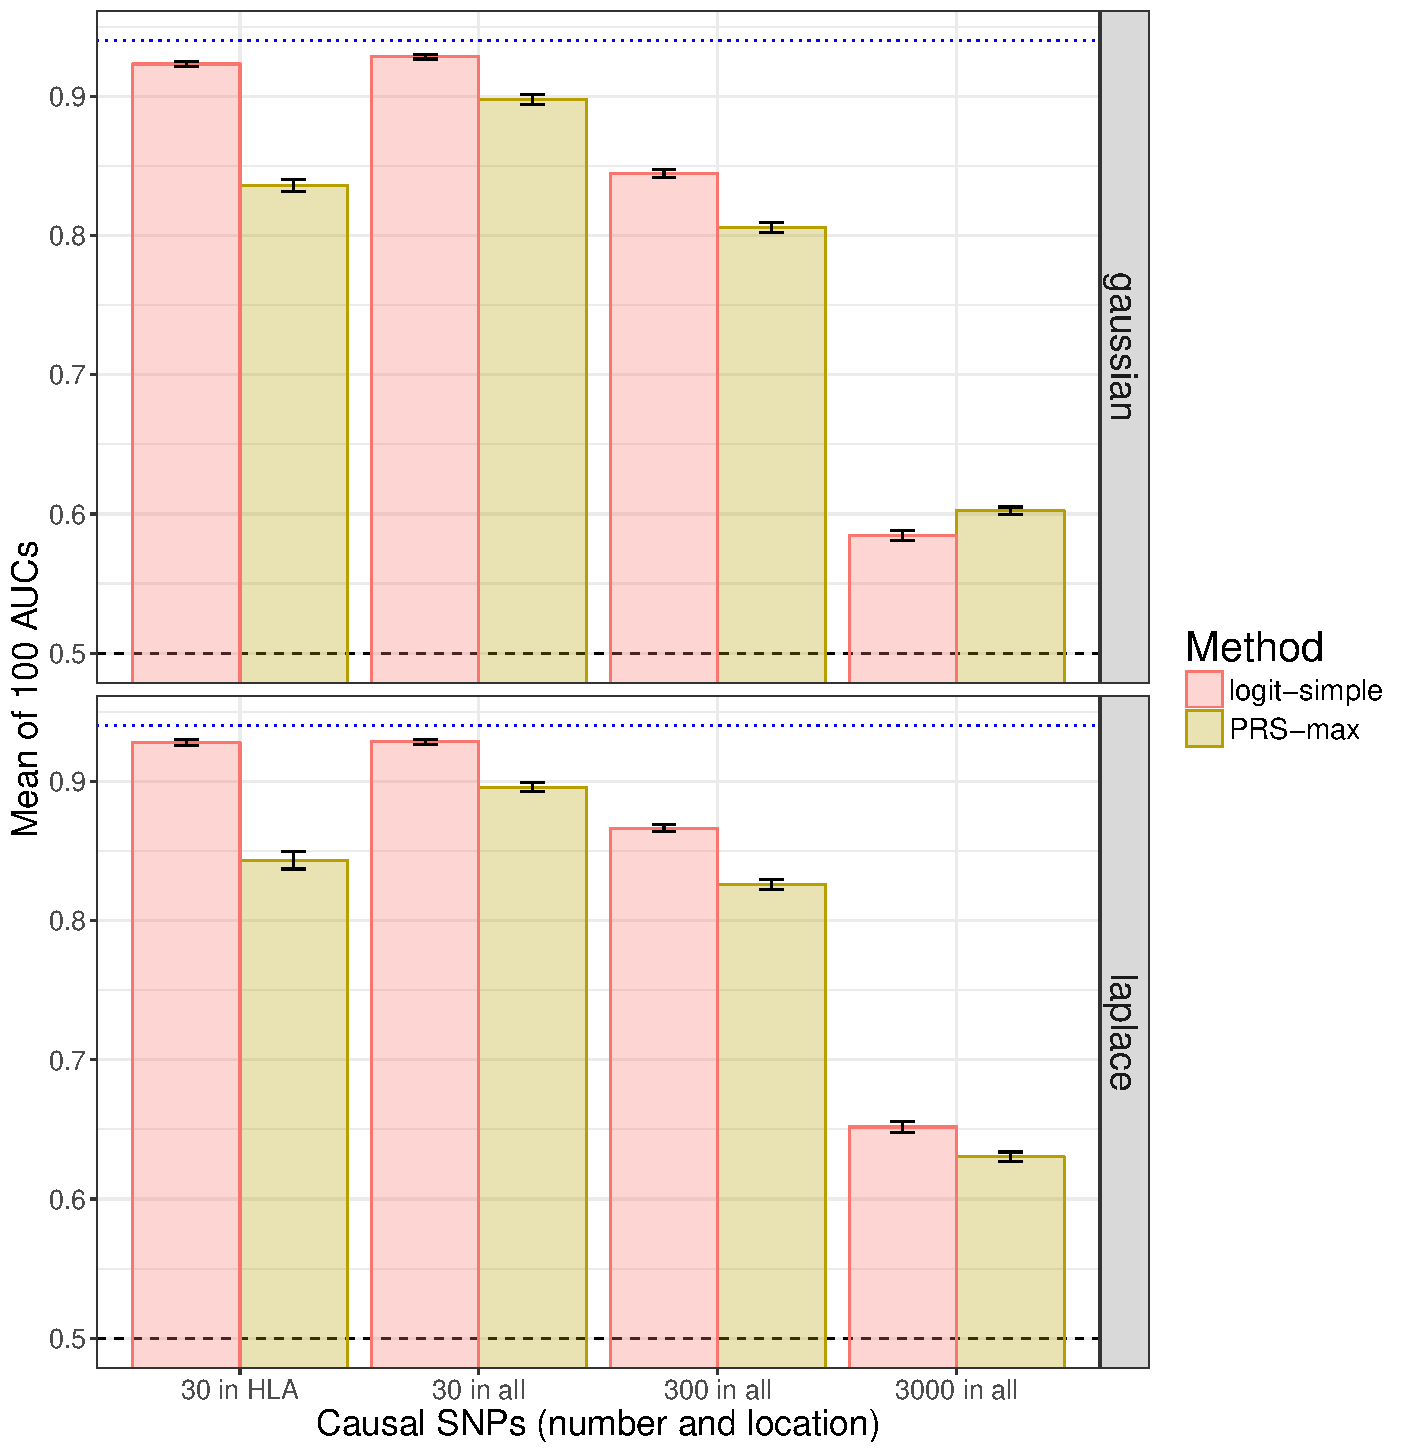
\includegraphics[width=\textwidth]{main-AUC-logit}}
\caption{Main comparison of the C+T method and ``logit-simple'' in scenario \textnumero1. Mean of AUC over 100 simulations for ``logit-simple'' and the maximum AUC reported with the C+T method (``PRS-max''). Upper (lower) panel is presenting results for effets following a Gaussian (Laplace) distribution. Error bars are representing $\pm 2 \text{SD}$ of $10^5$ non-parametric bootstrap of the mean of AUC. The blue dotted line represents the maximum achievable AUC. These results corresponds to the ``simple'' model and an heritability of 80\%.}
\label{fig:main-AUC-logit}
\end{figure}

\newpage
\begin{figure}[h]
\centerline{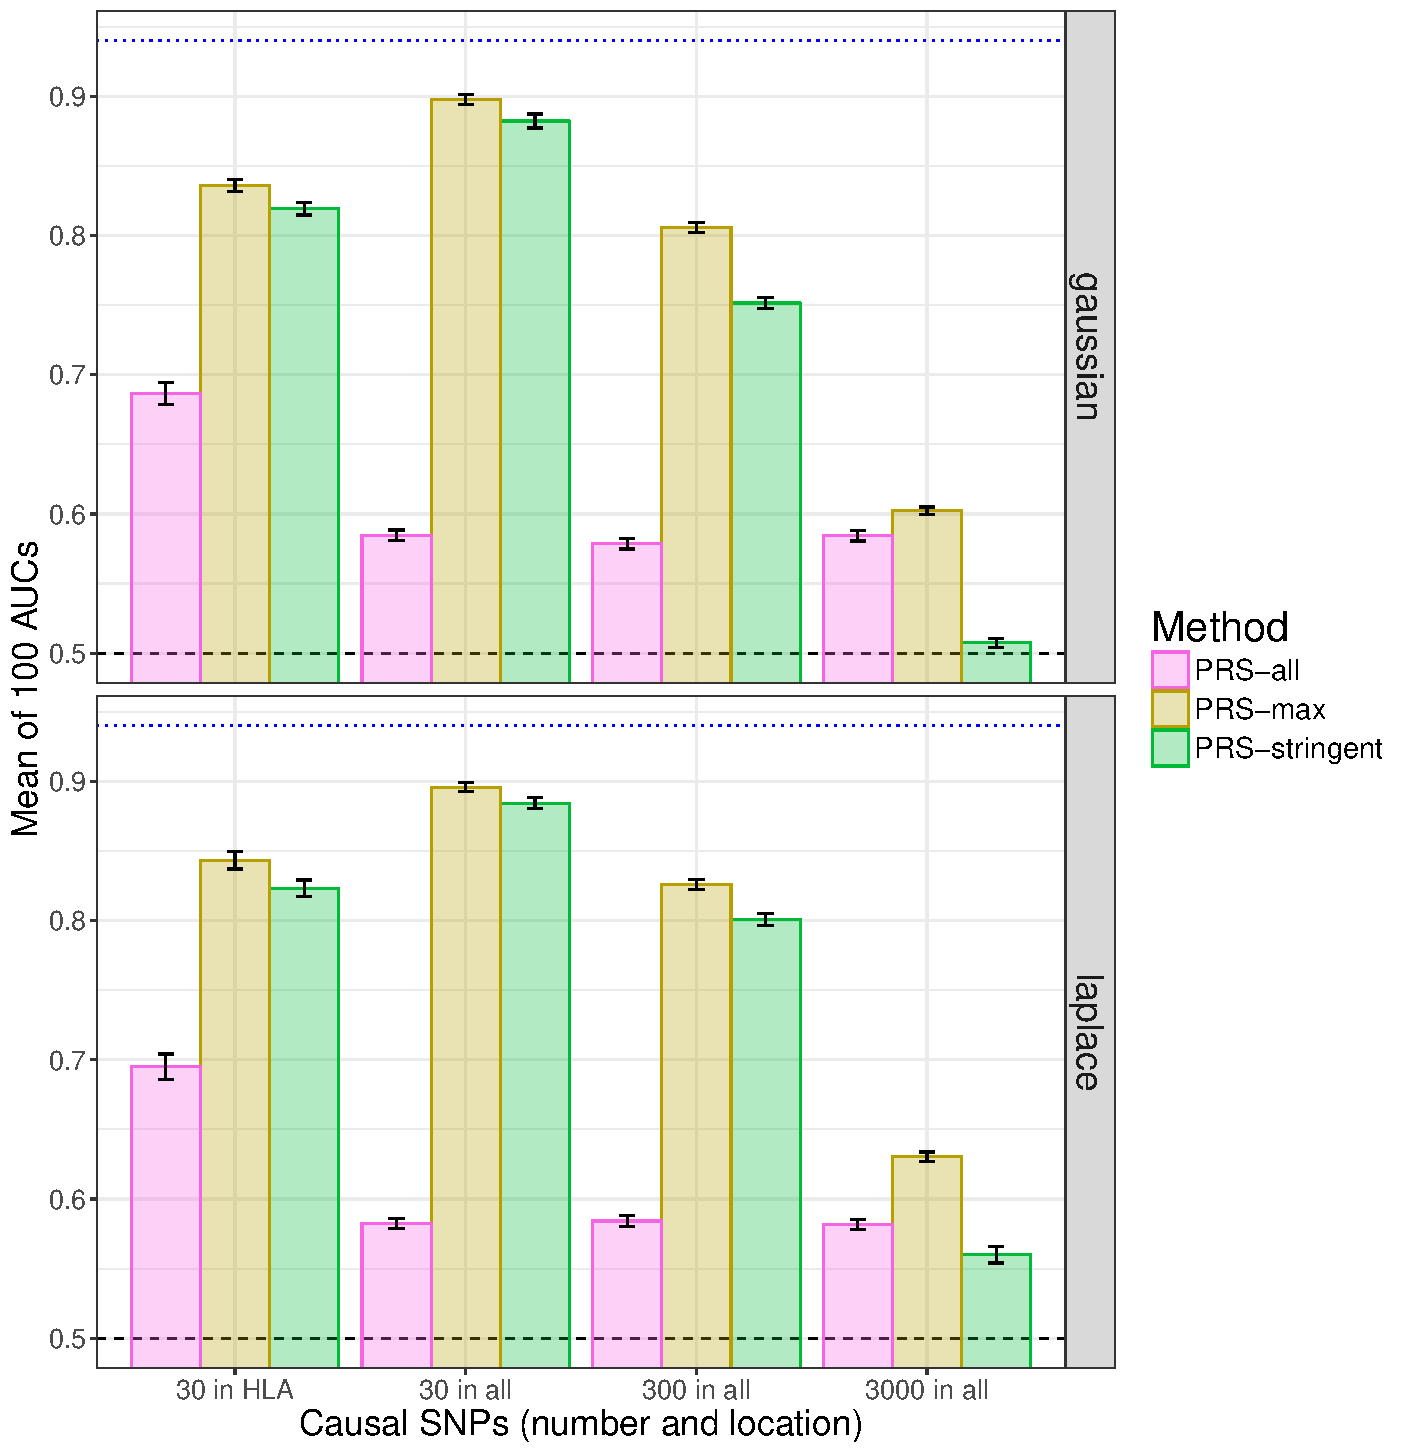
\includegraphics[width=\textwidth]{main-AUC-PRS}}
\caption{Comparison of three different threshold used in the C+T method in scenario \textnumero1. Mean of AUC over 100 simulations. Upper (lower) panel is presenting results for effets following a Gaussian (Laplace) distribution. Error bars are representing $\pm 2 \text{SD}$ of $10^5$ non-parametric bootstrap of the mean of AUC. The blue dotted line represents the maximum achievable AUC. These results corresponds to the ``simple'' model and an heritability of 80\%.}
\label{fig:main-AUC-PRS}
\end{figure}

\newpage
\begin{figure}[h]
\centerline{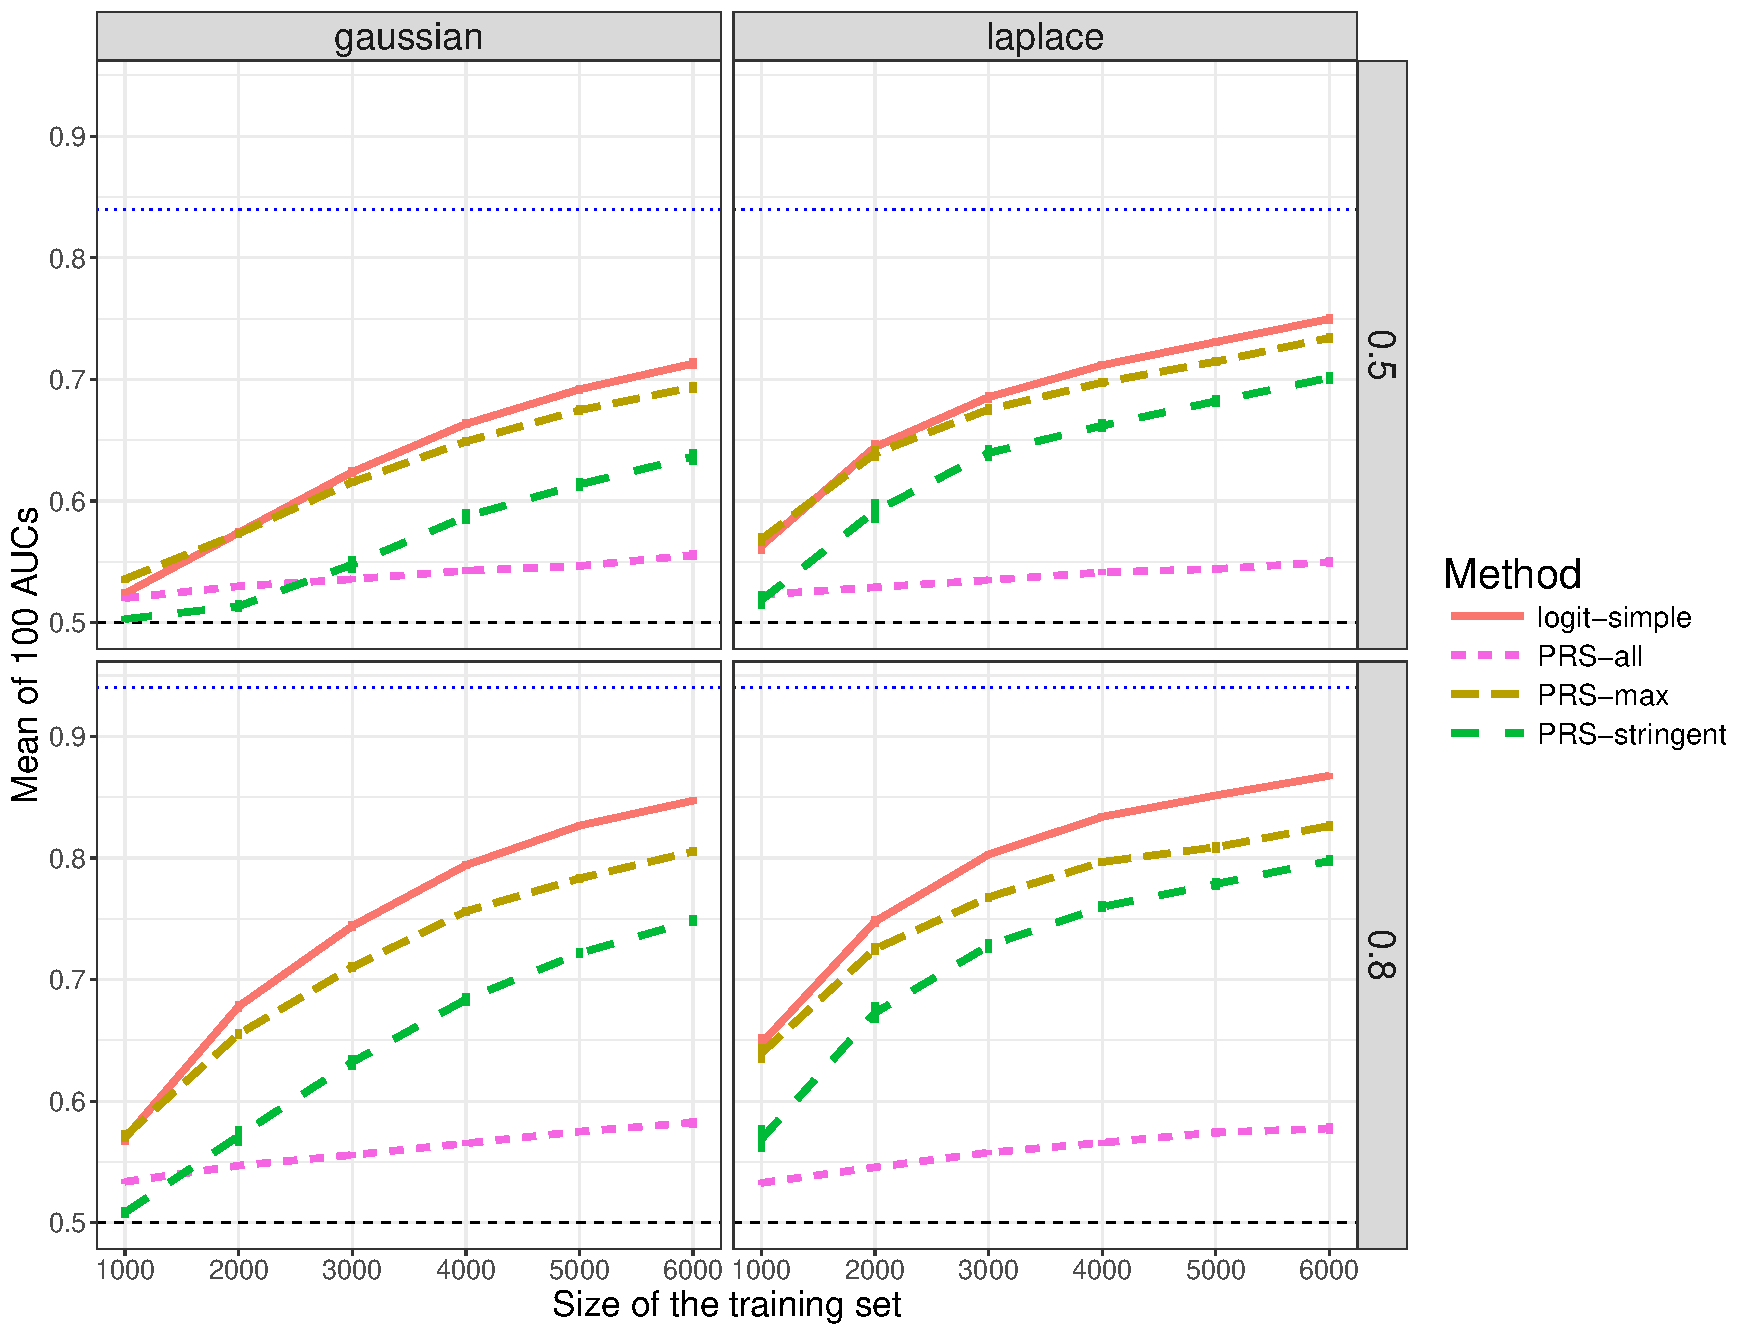
\includegraphics[width=\textwidth]{main-AUC-ntrain}}
\caption{Comparison of models when varying sample size in scenario \textnumero3. Mean of AUC over 100 simulations for ..the three reported PRSs... and the ``logit-simple'' as a function of the training size. These results are for the ``simple'' model with 300 causal SNPs sampled anywhere on the genome. Upper (lower) panels are presenting results for an heritability of 0.5 (0.8) and left (right) panels are presenting results for effets following a Gaussian (Laplace) distribution. Error bars are representing $\pm 2 \text{SD}$ of $10^5$ non-parametric bootstrap of the mean of AUC. The blue dotted line represents the maximum achievable AUC.}
\label{fig:main-AUC-ntrain}
\end{figure}

\newpage
\begin{figure}[h]
\centerline{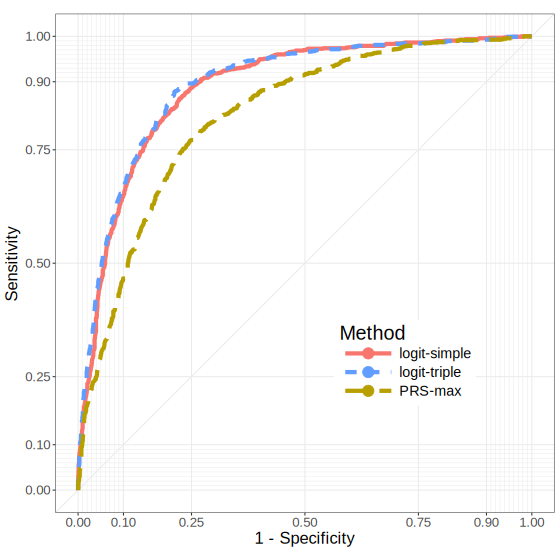
\includegraphics[width=\textwidth]{celiac-roc}}
\caption{ROC Curves for the ``C+T'', ``logit-simple'' and ``logit-triple'' methods for one run on the Celiac disease, training on 12,000 individuals and projecting on the remaining 3155 individuals. Plotted using R package plotROC \cite[]{sachs2017plotroc}.\label{fig:celiac-roc}}
\end{figure}

%%%%%%%%%%%%%%%%%%%%%%%%%%%%%%%%%%%%%%%%%%%%%%%%%%%%%%%%%%%%%%%%%%%%%%%%%%%%%%%%

\clearpage
\section*{Acknowledgements}

Authors acknowledge Grenoble Alpes Data Institute, supported by the French National Research Agency under the ``Investissements d'avenir'' program (ANR-15-IDEX-02) and the LabEx PERSYVAL-Lab (ANR-11-LABX-0025-01). We are also grateful to F\'elix Balazard for useful discussions about T-Trees, and to Yaohui Zeng for useful discussions about R package biglasso.

\vspace*{-12pt}

\bibliographystyle{natbib}
\bibliography{refs}

%%%%%%%%%%%%%%%%%%%%%%%%%%%%%%%%%%%%%%%%%%%%%%%%%%%%%%%%%%%%%%%%%%%%%%%%%%%%%%%%
%%%%%%%%%%%%%%%%%%%%%%%%%%%%%%%%%%%%%%%%%%%%%%%%%%%%%%%%%%%%%%%%%%%%%%%%%%%%%%%%
%%%%%%%%%%%%%%%%%%%%%%%%%%%%%%%%%%%%%%%%%%%%%%%%%%%%%%%%%%%%%%%%%%%%%%%%%%%%%%%%

\newpage
\section*{Supplementary Materials}

\renewcommand{\thefigure}{S\arabic{figure}}
\setcounter{figure}{0}
\renewcommand{\thetable}{S\arabic{table}}
\setcounter{table}{0}

%%%%%%%%%%%%%%%%%%%%%%%%%%%%%%%%%%%%%%%%%%%%%%%%%%%%%%%%%%%%%%%%%%%%%%%%%%%%%%%%

\subsection*{Maximum AUCs} \label{sec:auc-max}

We used three different ways to estimate the maximum achievable AUC for our simulations.
First, we used the estimation from equation (3) of \cite{wray2010genetic}. For a prevalence fixed at 30\% and an heritability of 50\% (respectively 80\%), the approximated theoretical values of AUC are 84.1\% (respectively 93.0\%). Note that this approximation is reported to be less accurate for high heritabilities.
Secondly, if we assume that the genetic part of the liabilities $y \sim N(0, h^2)$, we can estimate the theoretical value of the AUC that can be achieved given the heritability $h^2$ through Monte Carlo simulations. We report AUCs of 84.1\% and 94.1\% for respectively an heritability of 50\% and 80\%. [HOW TO ADD ERROR OF ESTIMATION? I HAVE SUMMARY() IN R]
Thirdly, we reproduce the exact same procedure of simulations and, for each combination of parameters (Table \ref{tab:simus}), we estimate the AUC of the ``oracle'', i.e.\ the true simulated genetic part of the liabilities through 100 replicates. For every combination of parameters, AUC of oracles are comprised between 83.2\% and 84.2\% for an heritability of 50\% and between 93.2\% and 94.1\% for an heritability of 80\%.
Given all these estimates of the maximal achievable AUC and for the sake of simplicity, we report maximum AUCs of 84\% (94\%) for heritabilities of 50\% (80\%) whatever are the parameters of the simulation.


%%%%%%%%%%%%%%%%%%%%%%%%%%%%%%%%%%%%%%%%%%%%%%%%%%%%%%%%%%%%%%%%%%%%%%%%%%%%%%%%

\newpage

\begin{table}[ht]
\centering
\begin{tabular}{|l|cccc|r|}
\hline
Population & UK & Finland & Netherlands & Italy & Total\\
\hline
Cases & 2569 & 637 & 795 & 495 & 4496\\
Controls & 7492 & 1799 & 828 & 540 & 10659\\
\hline
Total & 10061 & 2436 & 1623 & 1035 & 15155\\
\hline
\end{tabular}
\caption{Number of individuals by population and disease status in the celiac disease case-control study (after quality control, genotyped on 281,122 SNPs).\label{tab:celiac-data}}
\end{table}

%%%%%%%%%%%%%%%%%%%%%%%%%%%%%%%%%%%%%%%%%%%%%%%%%%%%%%%%%%%%%%%%%%%%%%%%%%%%%%%%

% latex table generated in R 3.4.1 by xtable 1.8-2 package
% Thu Oct 26 16:46:26 2017
\begin{table}[ht]
\centering
\begin{tabular}{ccccccccccccccc}
  \hline
1.00e+00 & 7.22e-01 & 5.87e-01 & 4.20e-01 & 2.43e-01 & 1.00e-01 & 2.35e-02 & 2.21e-03 & 4.69e-05 & 8.81e-08 & 3.18e-12 & 1.83e-19 & 2.89e-31 & 1.70e-50 & 7.71e-82 \\ 
  5.00e-08 & 7.05e-01 & 5.65e-01 & 3.95e-01 & 2.20e-01 & 8.47e-02 & 1.79e-02 & 1.42e-03 & 2.28e-05 & 2.73e-08 & 4.69e-13 & 8.08e-21 & 1.80e-33 & 4.30e-54 & 1.06e-87 \\ 
  7.94e-01 & 6.87e-01 & 5.42e-01 & 3.69e-01 & 1.97e-01 & 7.08e-02 & 1.34e-02 & 8.83e-04 & 1.05e-05 & 7.74e-09 & 6.03e-14 & 2.86e-22 & 7.73e-36 & 5.97e-58 & 5.49e-94 \\ 
  7.81e-01 & 6.69e-01 & 5.19e-01 & 3.43e-01 & 1.75e-01 & 5.85e-02 & 9.79e-03 & 5.31e-04 & 4.61e-06 & 2.01e-09 & 6.69e-15 & 7.92e-24 & 2.24e-38 & 4.37e-62 & 1.00e-100 \\ 
  7.67e-01 & 6.50e-01 & 4.95e-01 & 3.18e-01 & 1.54e-01 & 4.76e-02 & 7.01e-03 & 3.08e-04 & 1.90e-06 & 4.72e-10 & 6.32e-16 & 1.70e-25 & 4.26e-41 & 1.61e-66 &  \\ 
  7.53e-01 & 6.30e-01 & 4.70e-01 & 2.93e-01 & 1.35e-01 & 3.82e-02 & 4.90e-03 & 1.72e-04 & 7.31e-07 & 1.00e-10 & 5.04e-17 & 2.75e-27 & 5.16e-44 & 2.83e-71 &  \\ 
  7.38e-01 & 6.09e-01 & 4.46e-01 & 2.68e-01 & 1.17e-01 & 3.02e-02 & 3.33e-03 & 9.18e-05 & 2.63e-07 & 1.89e-11 & 3.35e-18 & 3.31e-29 & 3.84e-47 & 2.26e-76 &  \\ 
   \hline
\end{tabular}
\caption{The 102 thresholds used for the C+T method for this study.\label{tab:thr}}
\end{table}

%%%%%%%%%%%%%%%%%%%%%%%%%%%%%%%%%%%%%%%%%%%%%%%%%%%%%%%%%%%%%%%%%%%%%%%%%%%%%%%%

\newpage
\begin{figure}[h]
\centerline{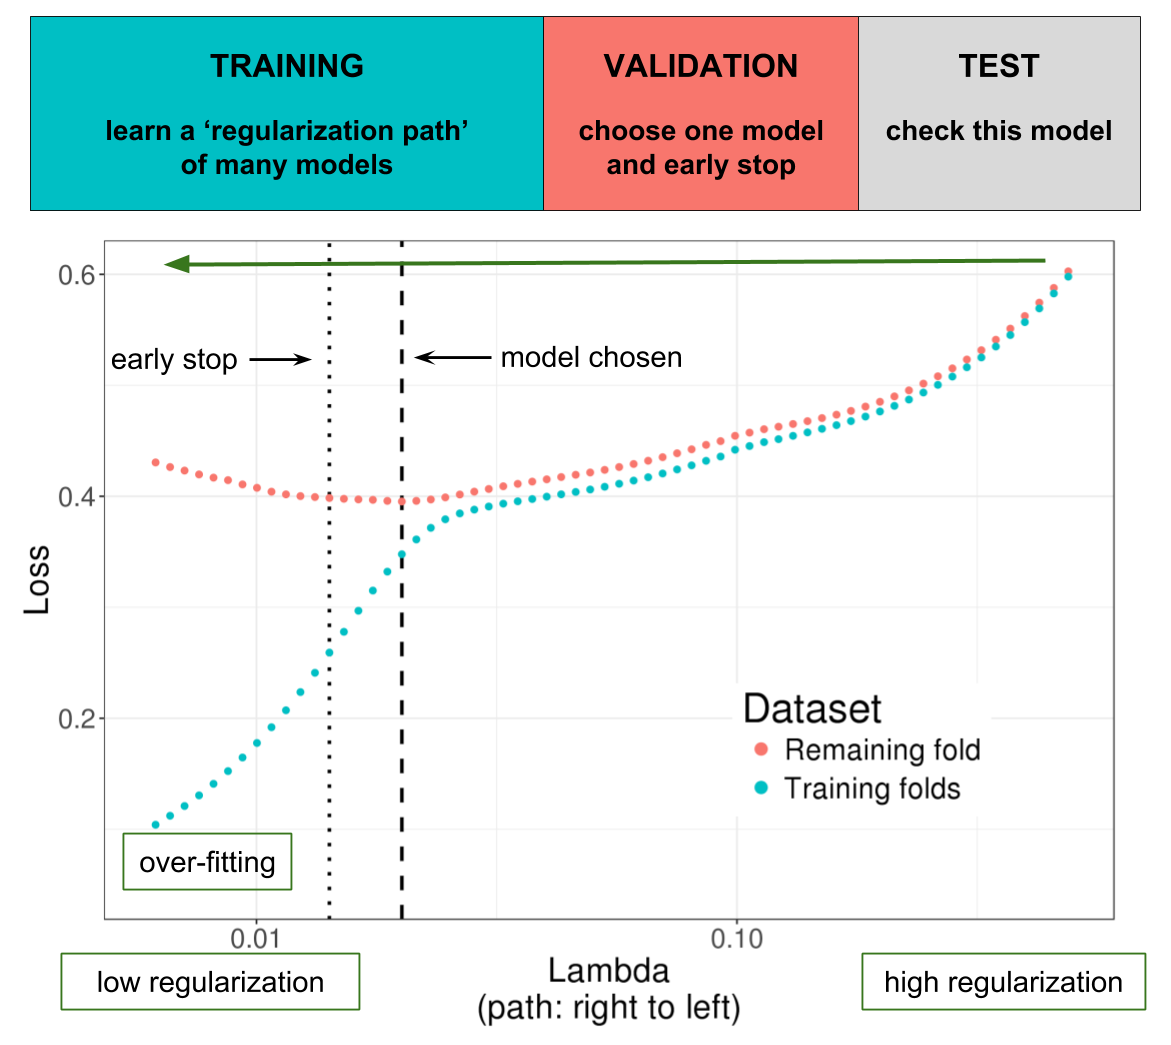
\includegraphics[width=\textwidth]{simple-CMSA}}
\caption{Illustration of one turn of the Cross-Model Selection and Averaging (CMSA) procedure. First, this procedure separates the training set in $K$ folds (e.g.\ 10 folds). 
Secondly, in turn, each fold is considered as an inner validation set (red) and the other ($K - 1$) folds form an inner training set (blue). A ``regularization path'' of models is trained on the inner training set and the corresponding predictions (scores) for the inner validation set are computed. The model that minimizes the loss on the inner validation set is selected. Finally, the $K$ resulting models are averaged. 
We also use this procedure to derive an early stopping criterion so that the algorithm does not need to evaluate the whole regularization paths, making this procedure much faster.}
\label{fig:CMSA}
\end{figure}

%%%%%%%%%%%%%%%%%%%%%%%%%%%%%%%%%%%%%%%%%%%%%%%%%%%%%%%%%%%%%%%%%%%%%%%%%%%%%%%%

\newpage
\begin{figure}[h]
\centerline{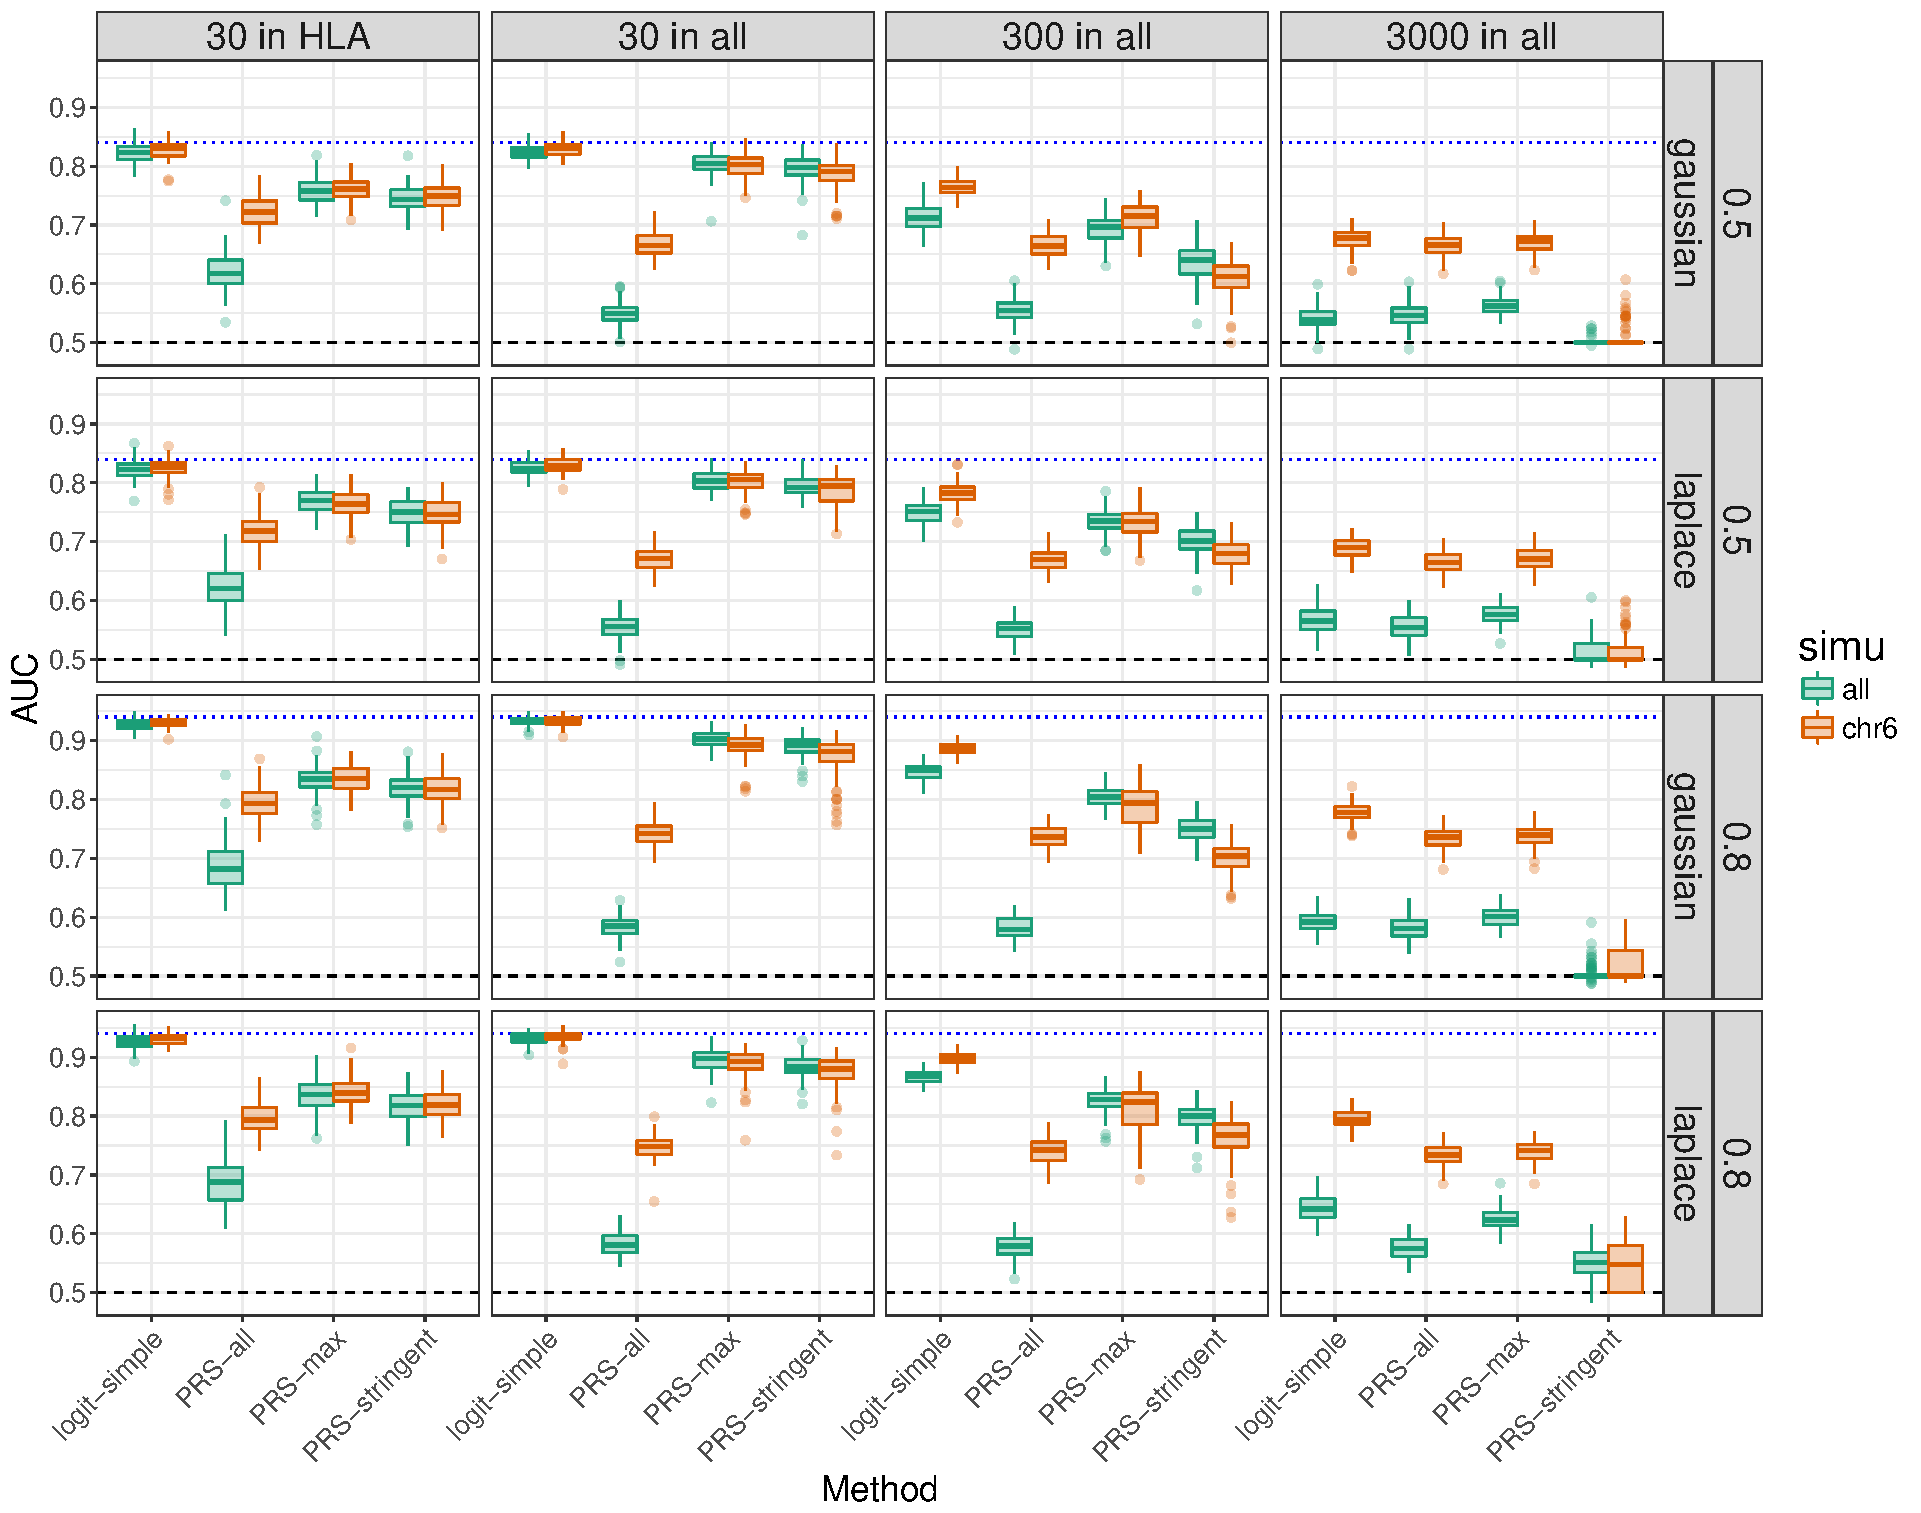
\includegraphics[width=\textwidth]{supp-AUC-chr6}}
\caption{Comparison of models when using only chromosome 6 in scenario \textnumero2. Boxplots of AUC over 100 simulations for ..the three reported PRSs... and the ``logit-simple''.
Vertical panels represents different number of causal SNPs and their location (``all'': anywhere on the genome; ``HLA'': only in the HLA region). Horizontal panels are presenting results for effets following a Gaussian or Laplace distribution and an heritability of 0.5 or 0.8. The blue dotted line represents the maximum achievable AUC. The ``simple'' model was used to simulate phenotypes.}
\label{fig:supp-AUC-chr6}
\end{figure}

%%%%%%%%%%%%%%%%%%%%%%%%%%%%%%%%%%%%%%%%%%%%%%%%%%%%%%%%%%%%%%%%%%%%%%%%%%%%%%%%

\newpage
\begin{figure}[h]
\centerline{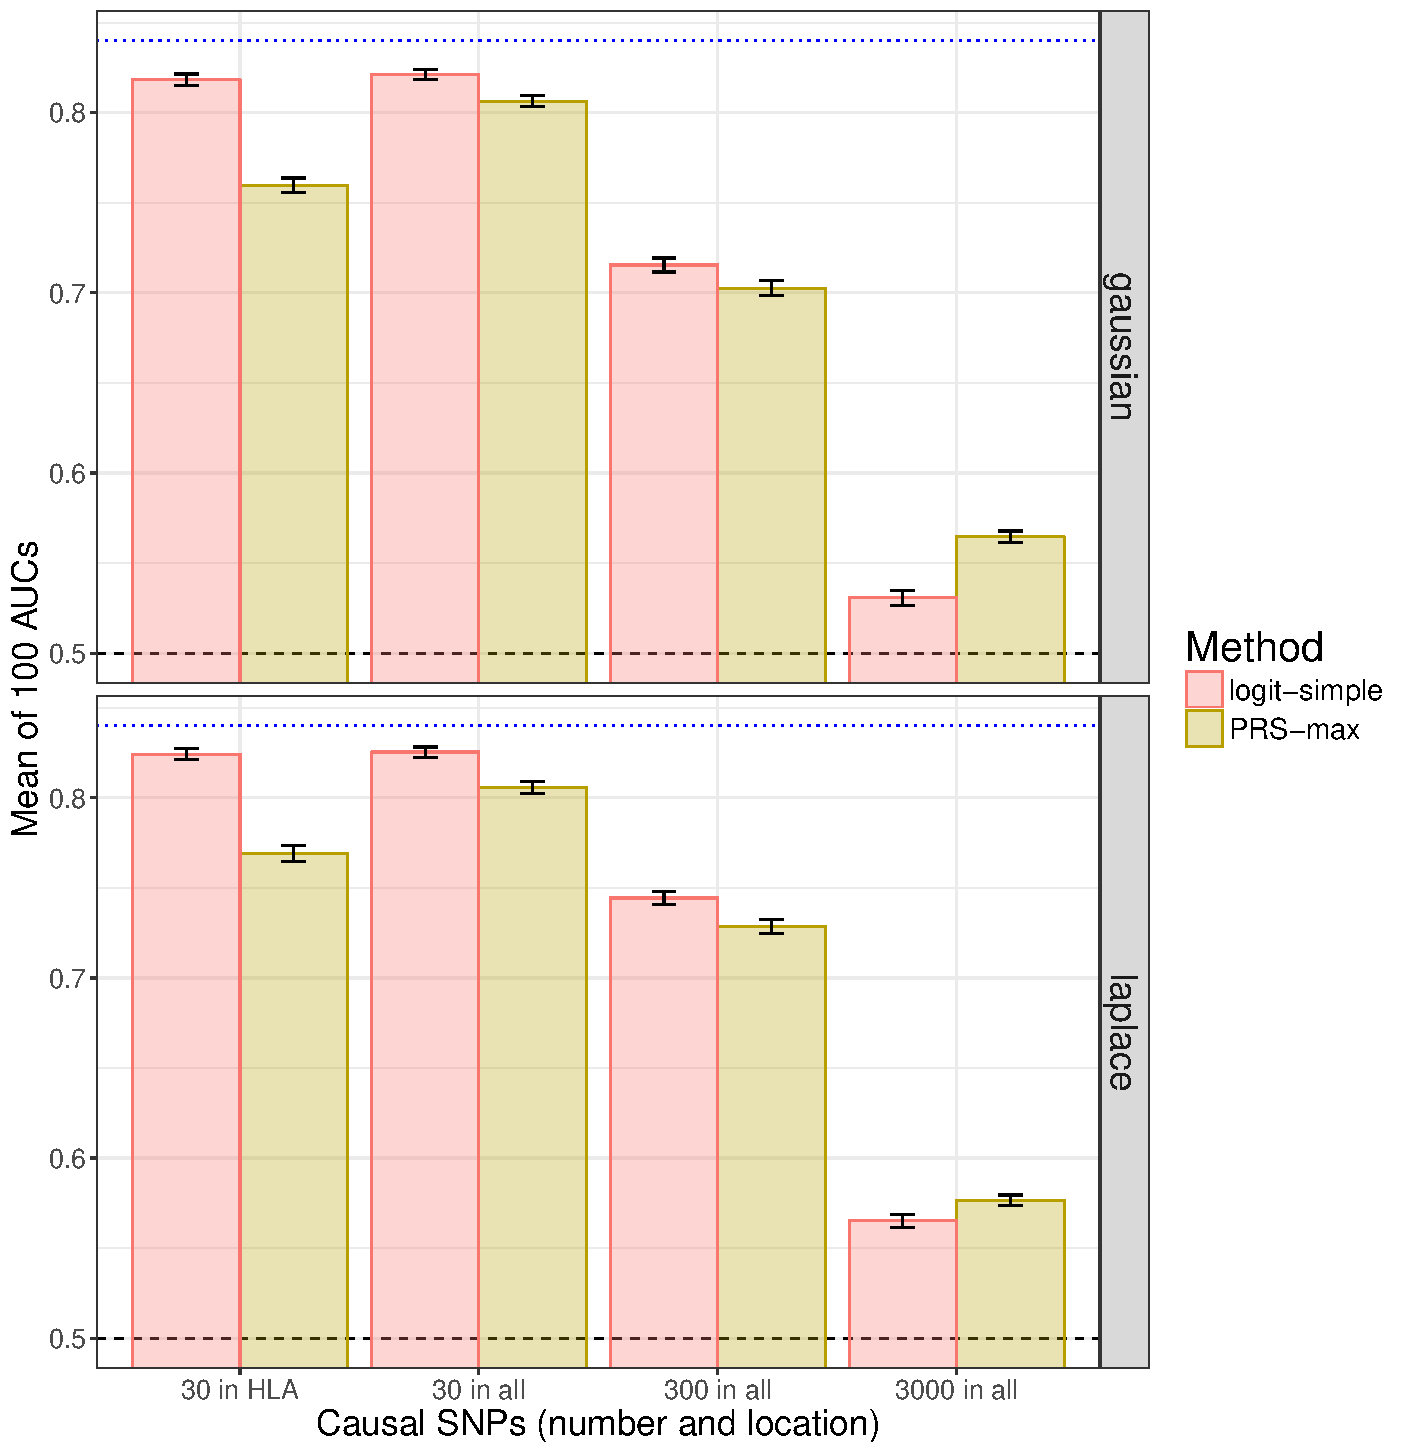
\includegraphics[width=\textwidth]{supp-AUC-logit}}
\caption{[COPY FOR H2=0.5]}
\label{fig:supp-AUC-logit}
\end{figure}

\newpage
\begin{figure}[h]
\centerline{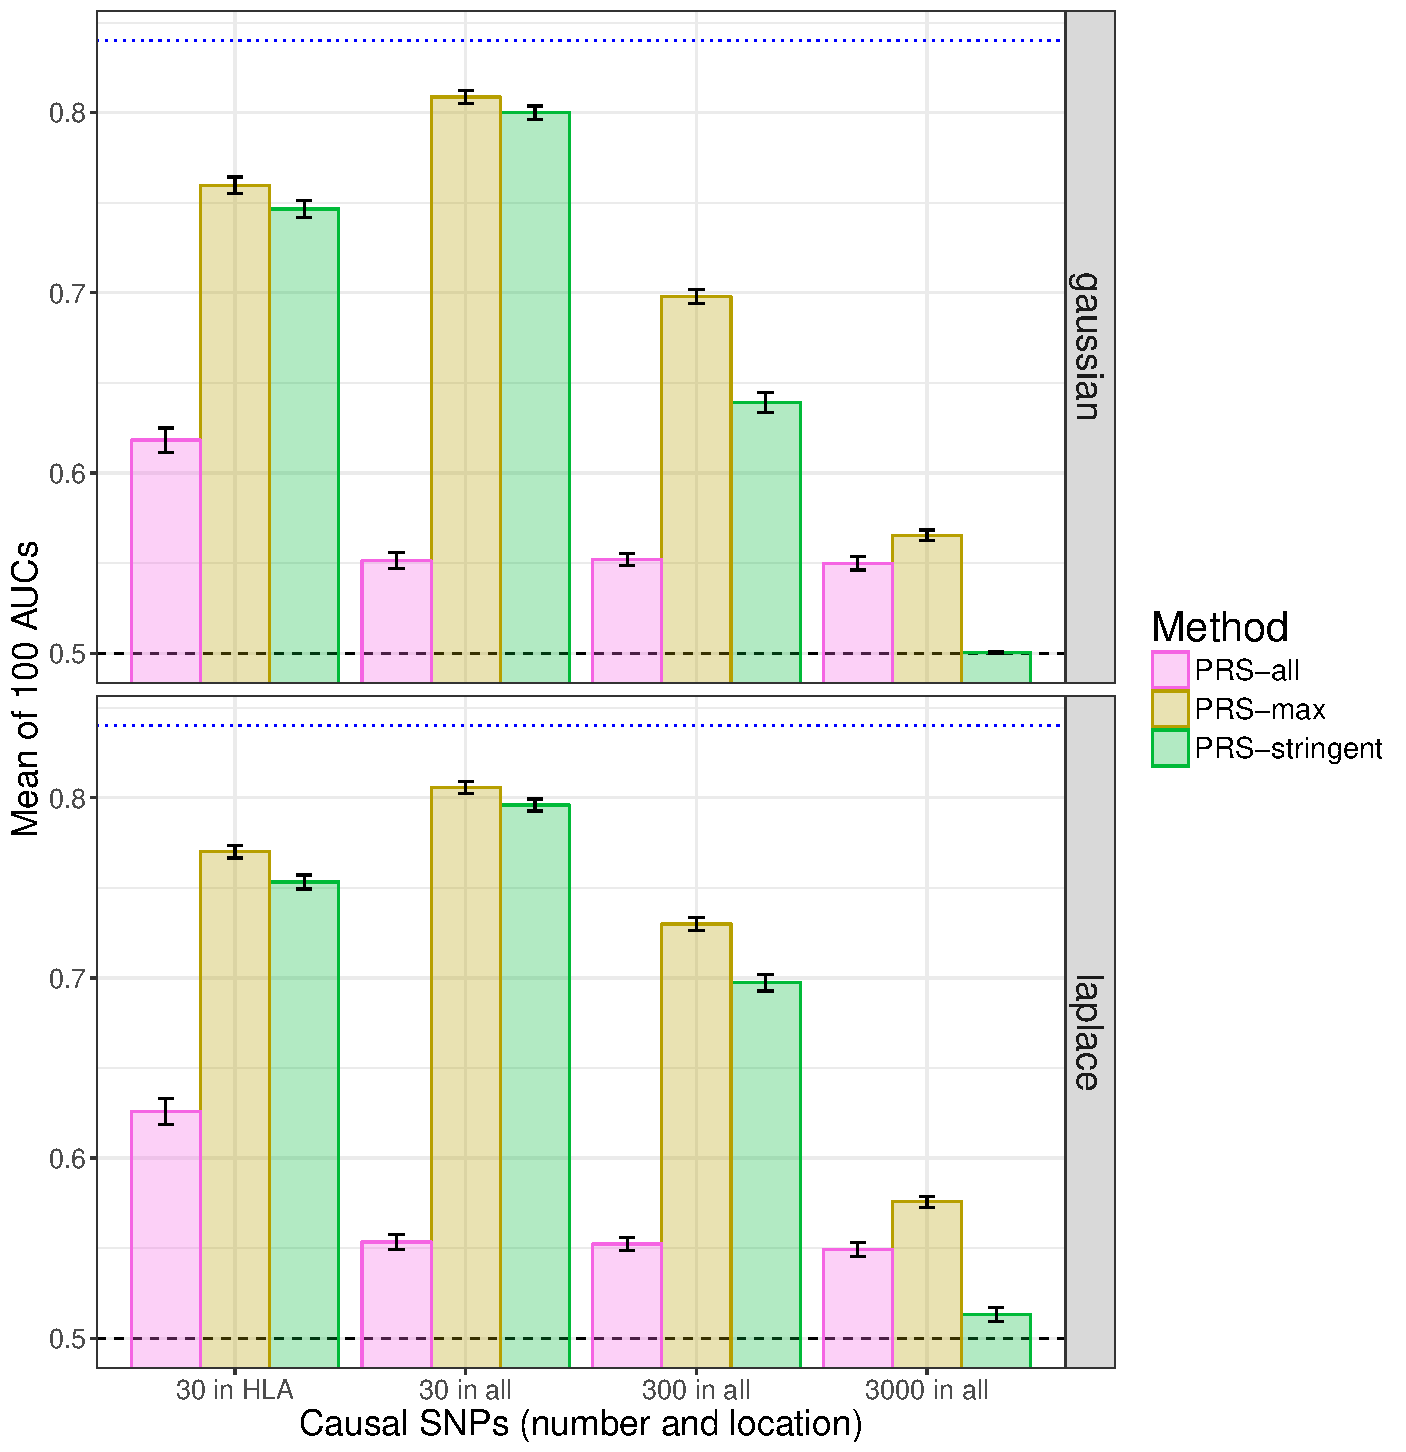
\includegraphics[width=\textwidth]{supp-AUC-PRS}}
\caption{[COPY FOR H2=0.5]}
\label{fig:supp-AUC-PRS}
\end{figure}

%%%%%%%%%%%%%%%%%%%%%%%%%%%%%%%%%%%%%%%%%%%%%%%%%%%%%%%%%%%%%%%%%%%%%%%%%%%%%%%%

\newpage
\begin{figure}[h]
\centerline{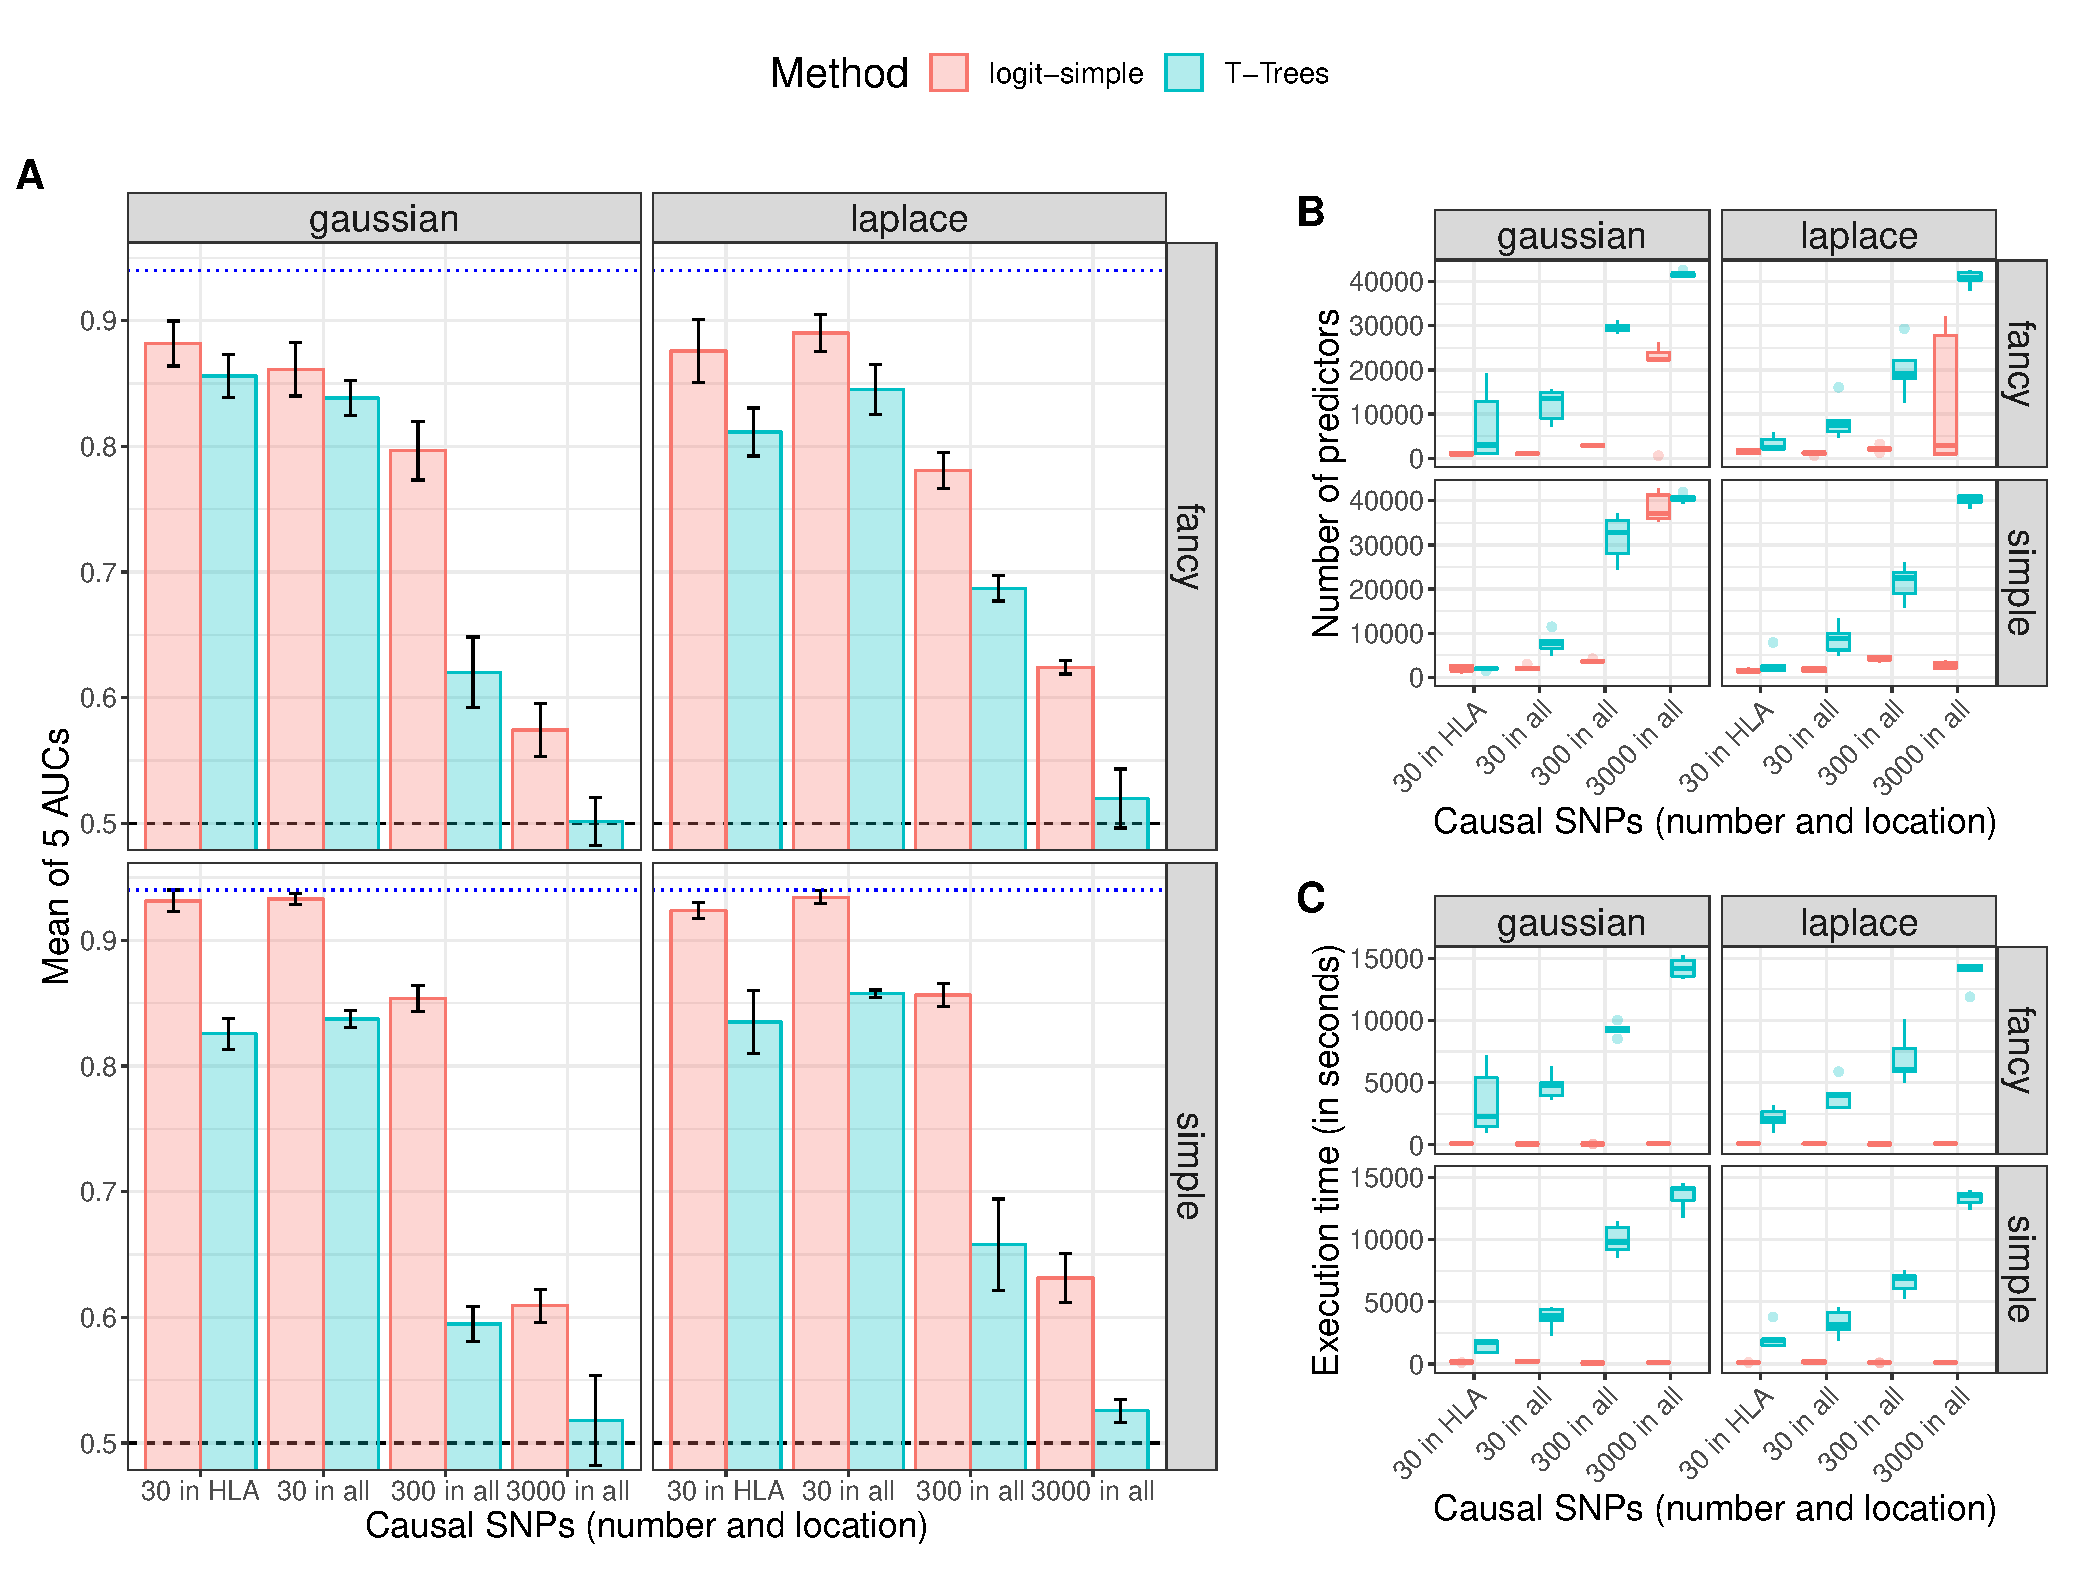
\includegraphics[width=\textwidth]{supp-ttrees}}
\caption{Comparison of T-Trees and ``logit-simple'' in scenario \textnumero1. Vertical panels are presenting results for effects following a Gaussian or Laplace distribution. Horizontal panels are presenting results for the ``simple'' and ``fancy'' models for simulating phenotypes. Simulations use an heritability of 80\%. \textbf{A:} Mean of AUC over 5 simulations. Error bars are representing $\pm 2 \text{SD}$ of $10^5$ non-parametric bootstrap of the mean of AUC. The blue dotted line represents the maximum achievable AUC. \textbf{B:} Boxplots of numbers of predictors used by the methods for 5 simulations. \textbf{C:} Boxplots of execution times for 5 simulations.}
\label{fig:supp-ttrees}
\end{figure}

\newpage
\begin{figure}[h]
\centerline{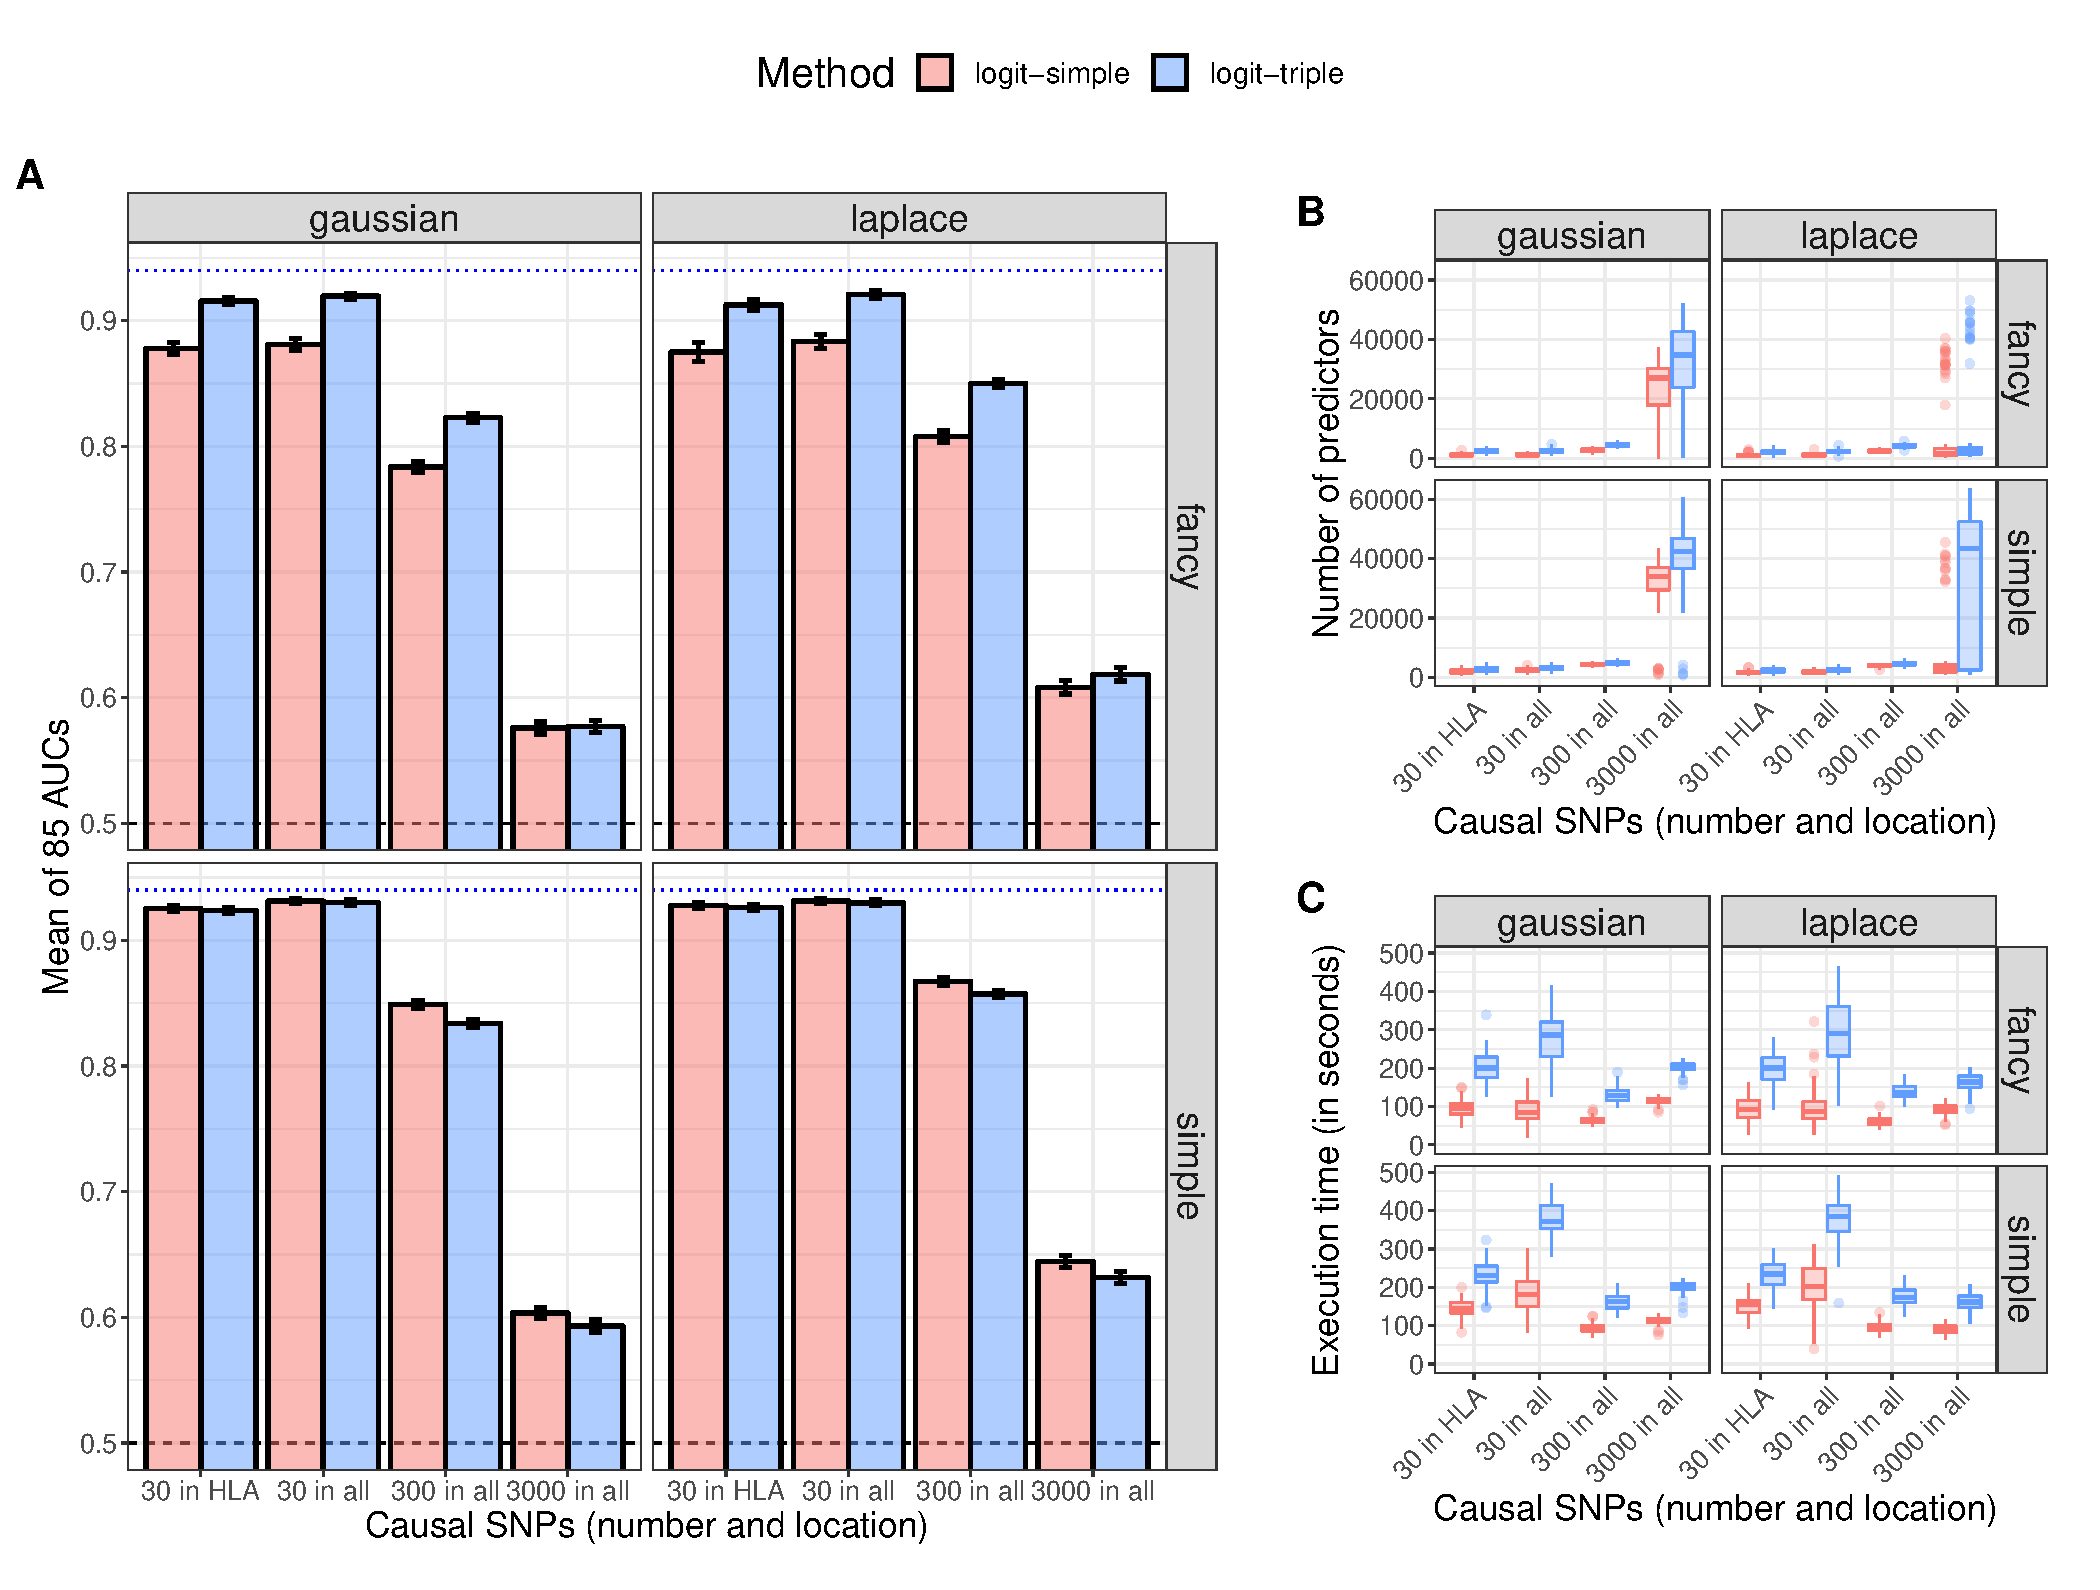
\includegraphics[width=\textwidth]{supp-triple}}
\caption{Comparison of ``logit-triple'' and ``logit-simple'' in scenario \textnumero1. Vertical panels are presenting results for effects following a Gaussian or Laplace distribution. Horizontal panels are presenting results for the ``simple'' and ``fancy'' models for simulating phenotypes. Simulations use an heritability of 80\%. \textbf{A:} Mean of AUC over 100 simulations. Error bars are representing $\pm 2 \text{SD}$ of $10^5$ non-parametric bootstrap of the mean of AUC. The blue dotted line represents the maximum achievable AUC. \textbf{B:} Boxplots of numbers of predictors used by the methods for 100 simulations. \textbf{C:} Boxplots of execution times for 100 simulations.}
\label{fig:supp-triple}
\end{figure}

\newpage
\begin{figure}[h]
\centerline{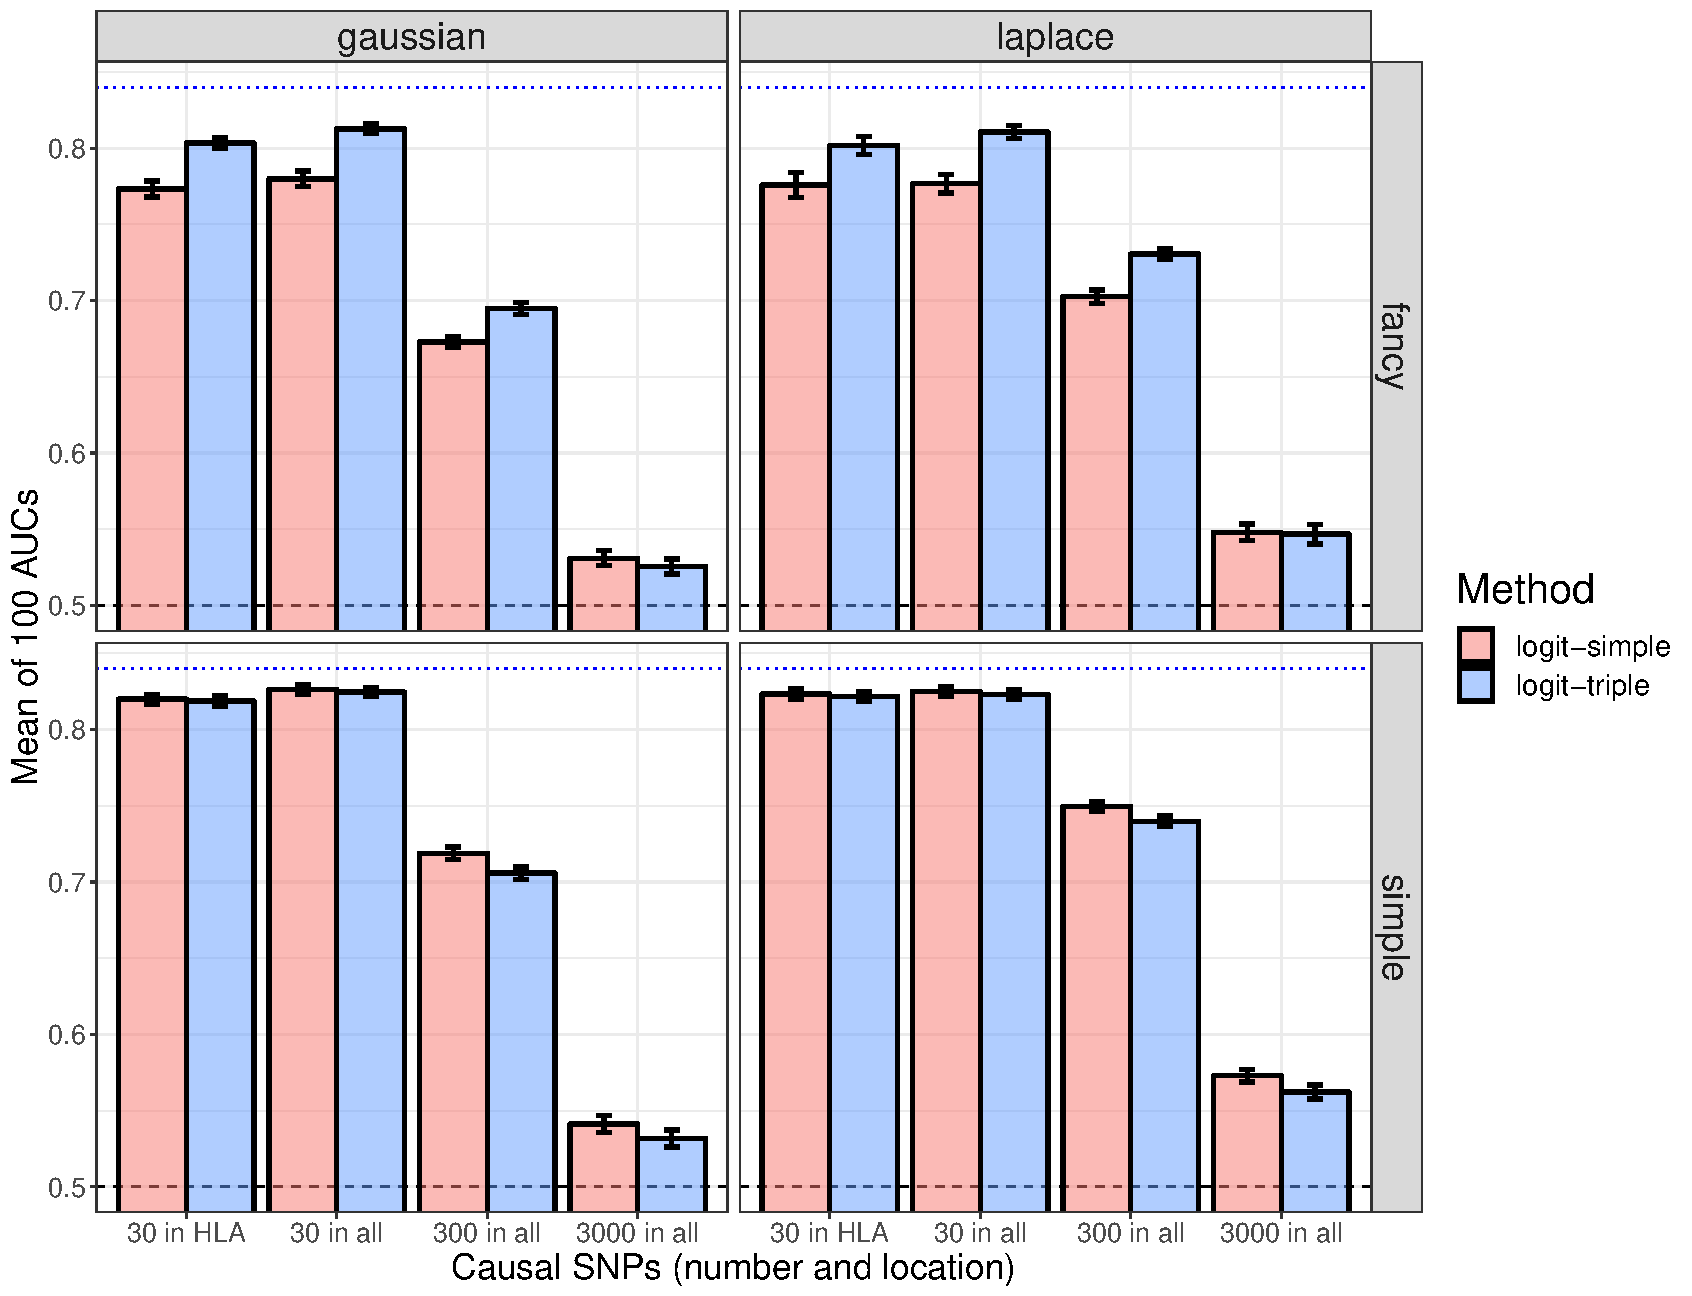
\includegraphics[width=\textwidth]{supp-AUC-triple}}
\caption{[TRIPLE ONLY AUC - H2=0.5]}
\label{fig:supp-AUC-triple}
\end{figure}

\newpage
\begin{figure}[h]
\centerline{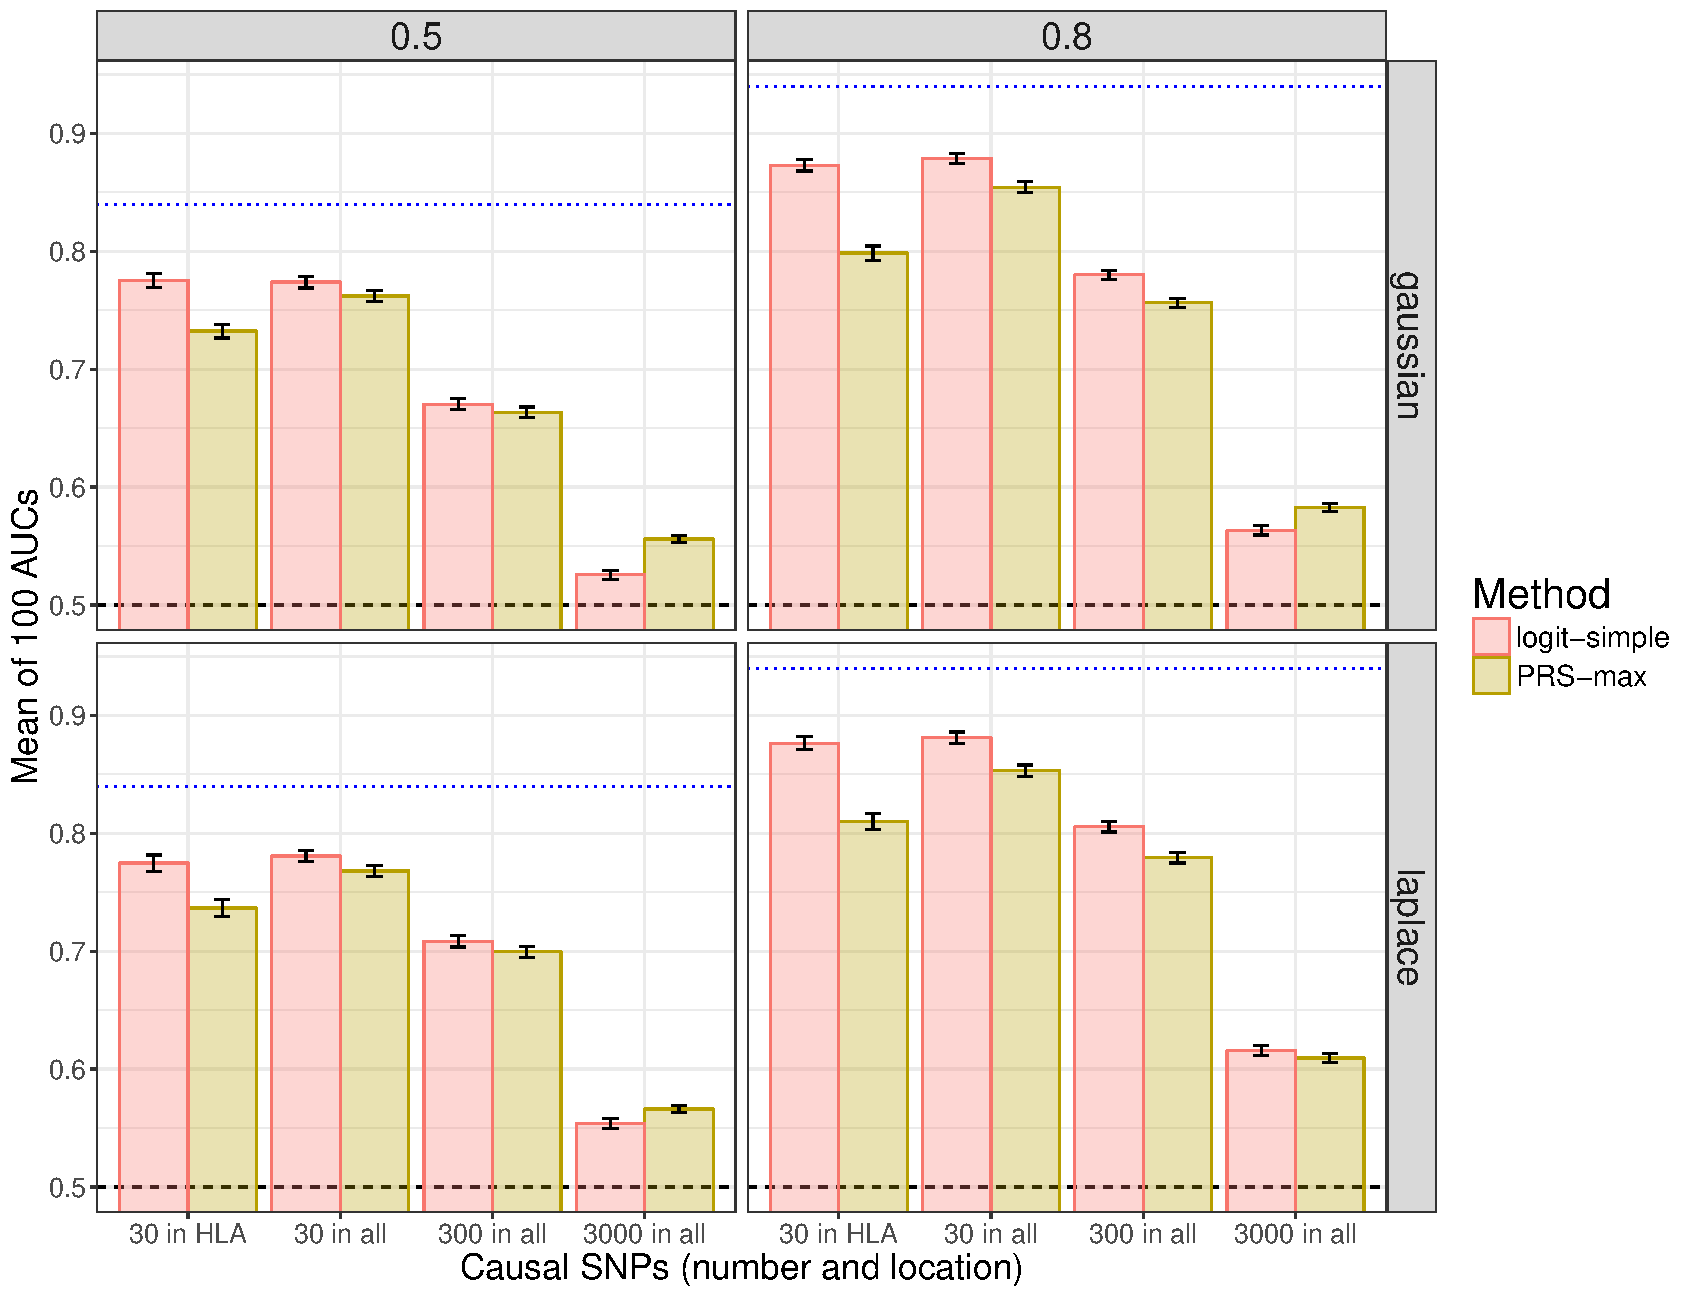
\includegraphics[width=\textwidth]{supp-AUC-logit-fancy}}
\caption{[COPY FOR H2=0.5 \& MODEL FANCY]}
\label{fig:supp-AUC-logit-fancy}
\end{figure}

\newpage
\begin{figure}[h]
\centerline{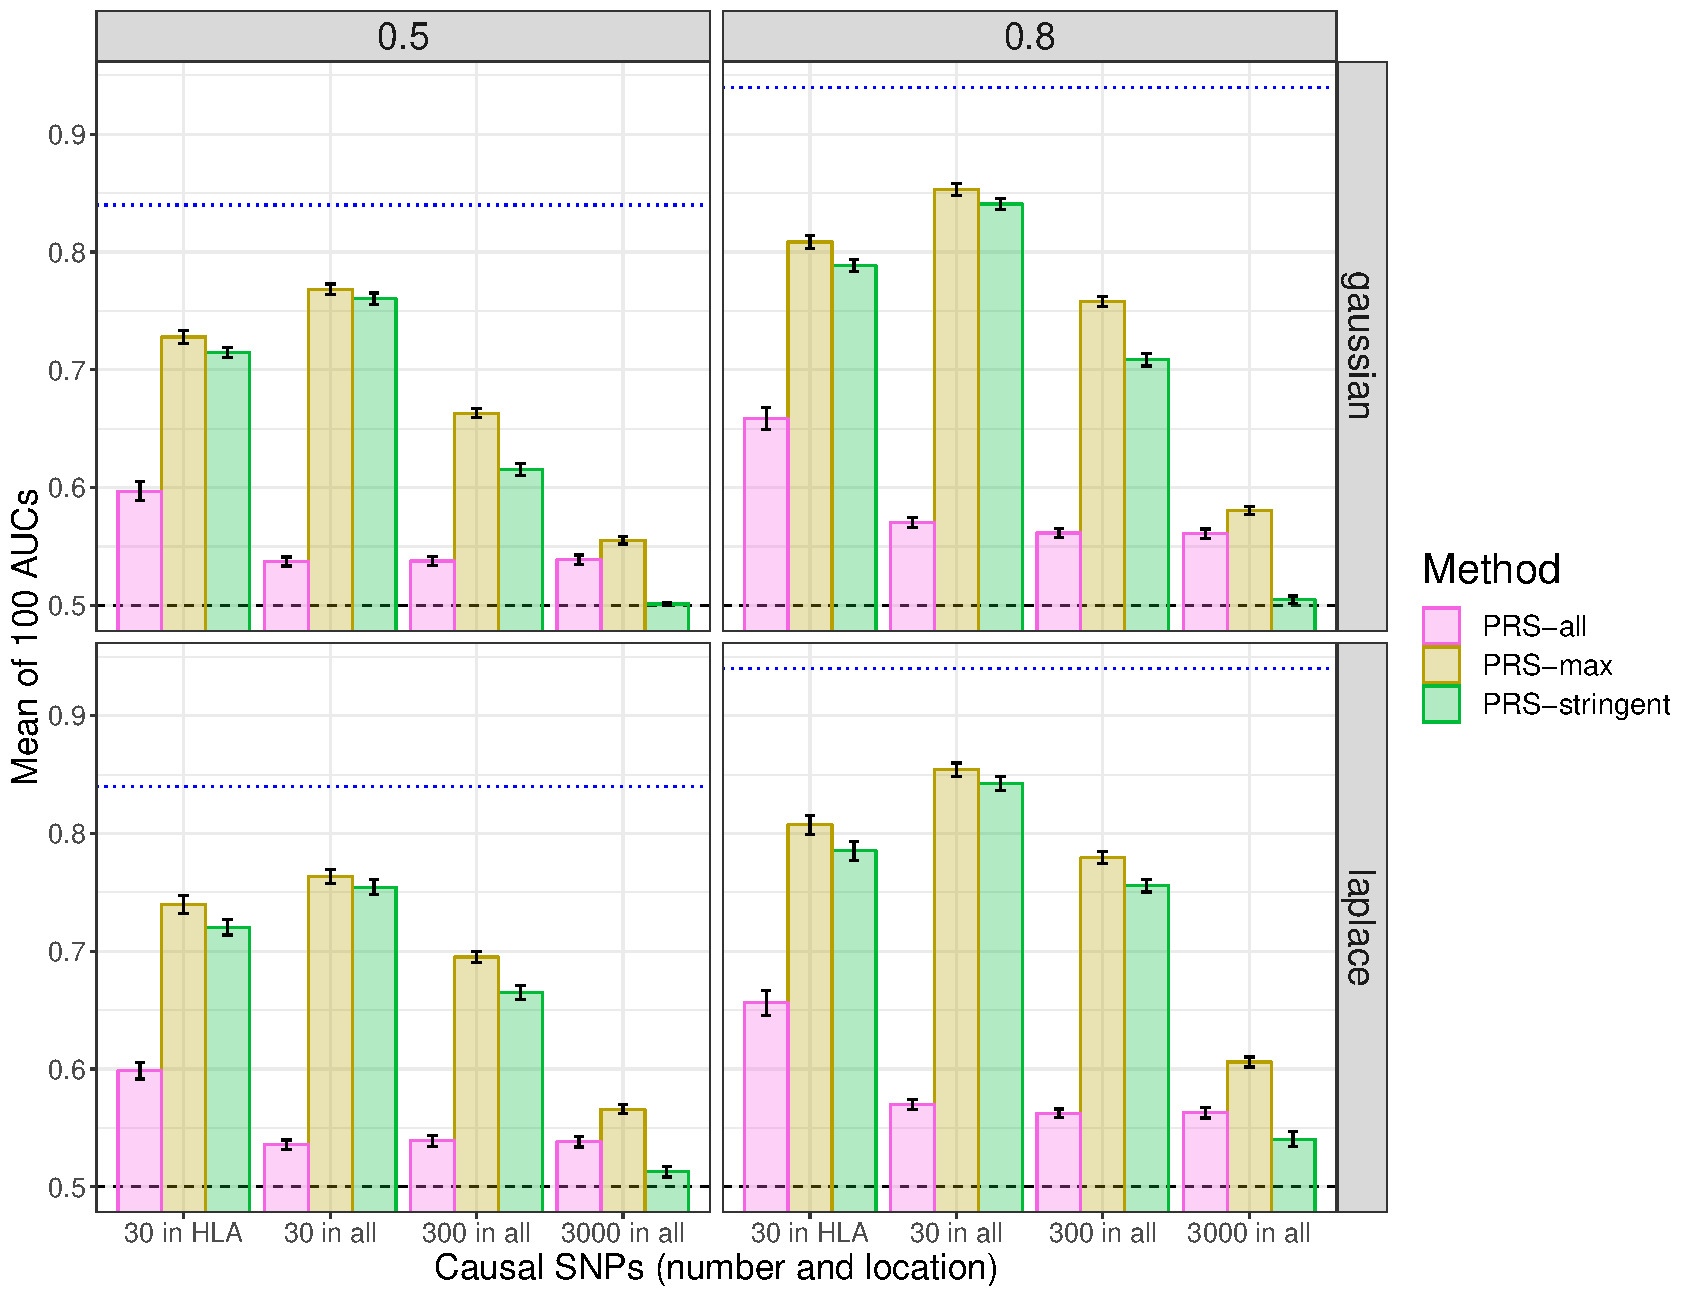
\includegraphics[width=\textwidth]{supp-AUC-PRS-fancy}}
\caption{[COPY FOR H2=0.5 \& MODEL FANCY]}
\label{fig:supp-AUC-PRS-fancy}
\end{figure}

%%%%%%%%%%%%%%%%%%%%%%%%%%%%%%%%%%%%%%%%%%%%%%%%%%%%%%%%%%%%%%%%%%%%%%%%%%%%%%%%

\newpage
\begin{figure}[h]
\centerline{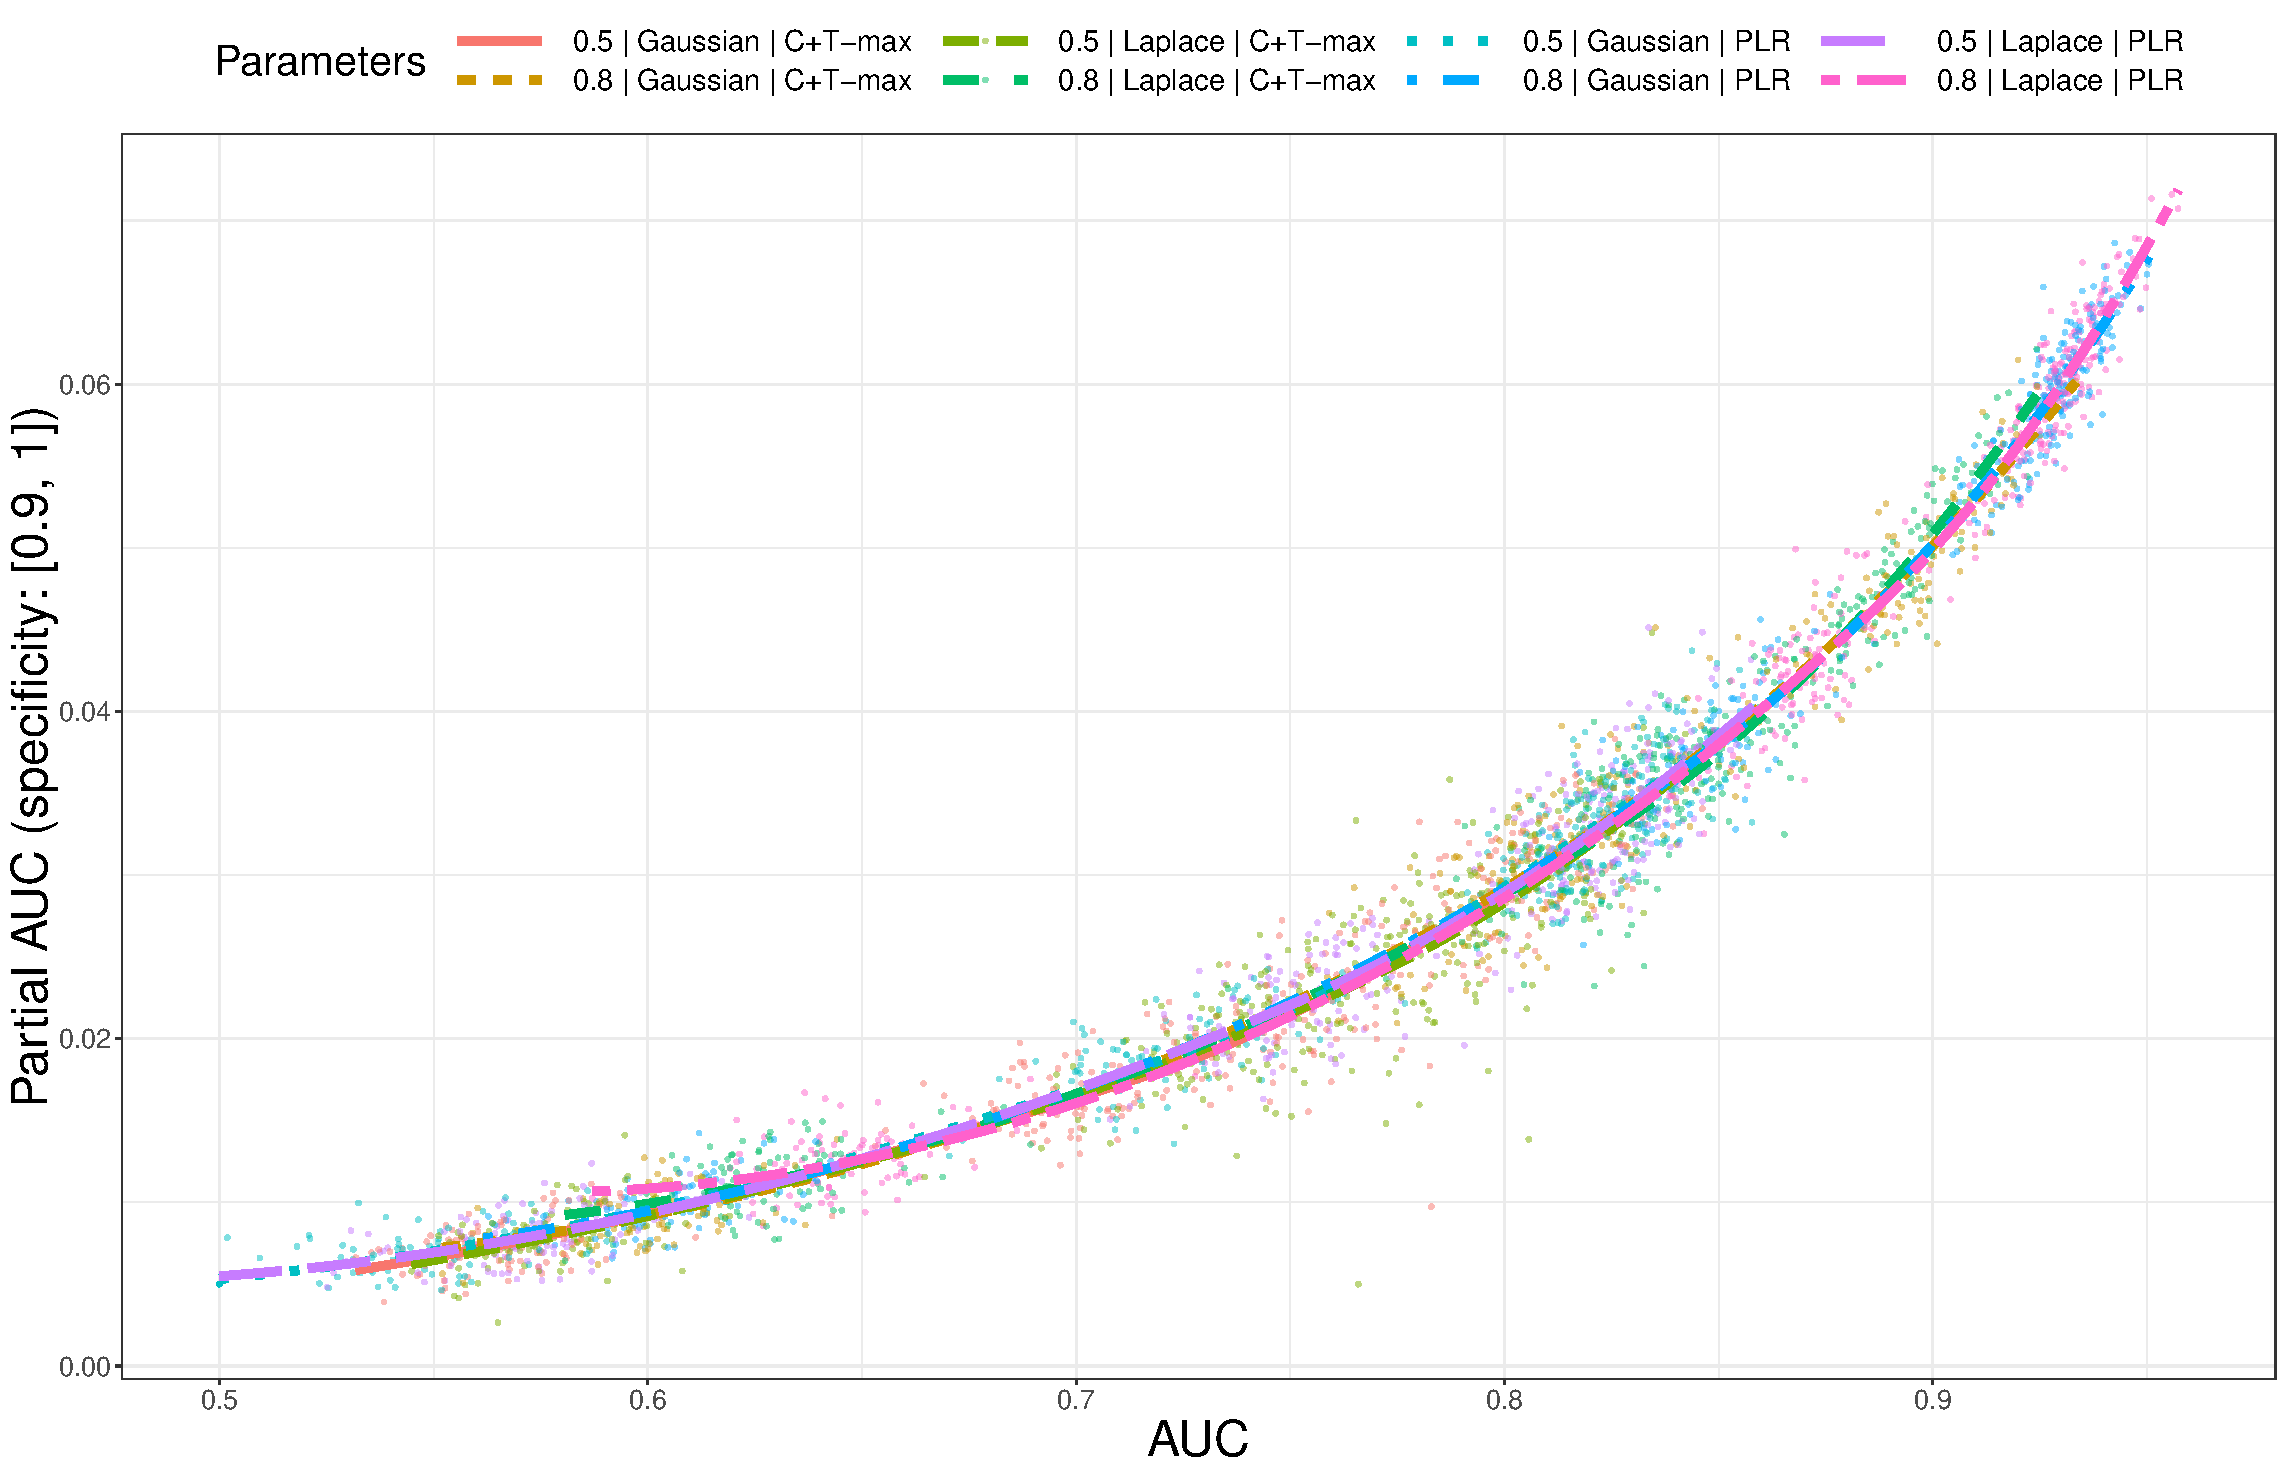
\includegraphics[width=\textwidth]{supp-AUC-corr}}
\caption{Correlation between AUC and partial AUC values in scenario \textnumero1. There is a Spearman correlation of 98\% between values of AUC and partial AUC. The relation between the two values are the same whatever are the heritability, distribution of effects and method used.\label{fig:supp-AUC-corr}}
\end{figure}

%%%%%%%%%%%%%%%%%%%%%%%%%%%%%%%%%%%%%%%%%%%%%%%%%%%%%%%%%%%%%%%%%%%%%%%%%%%%%%%%

\newpage
\begin{figure}[h]
\centerline{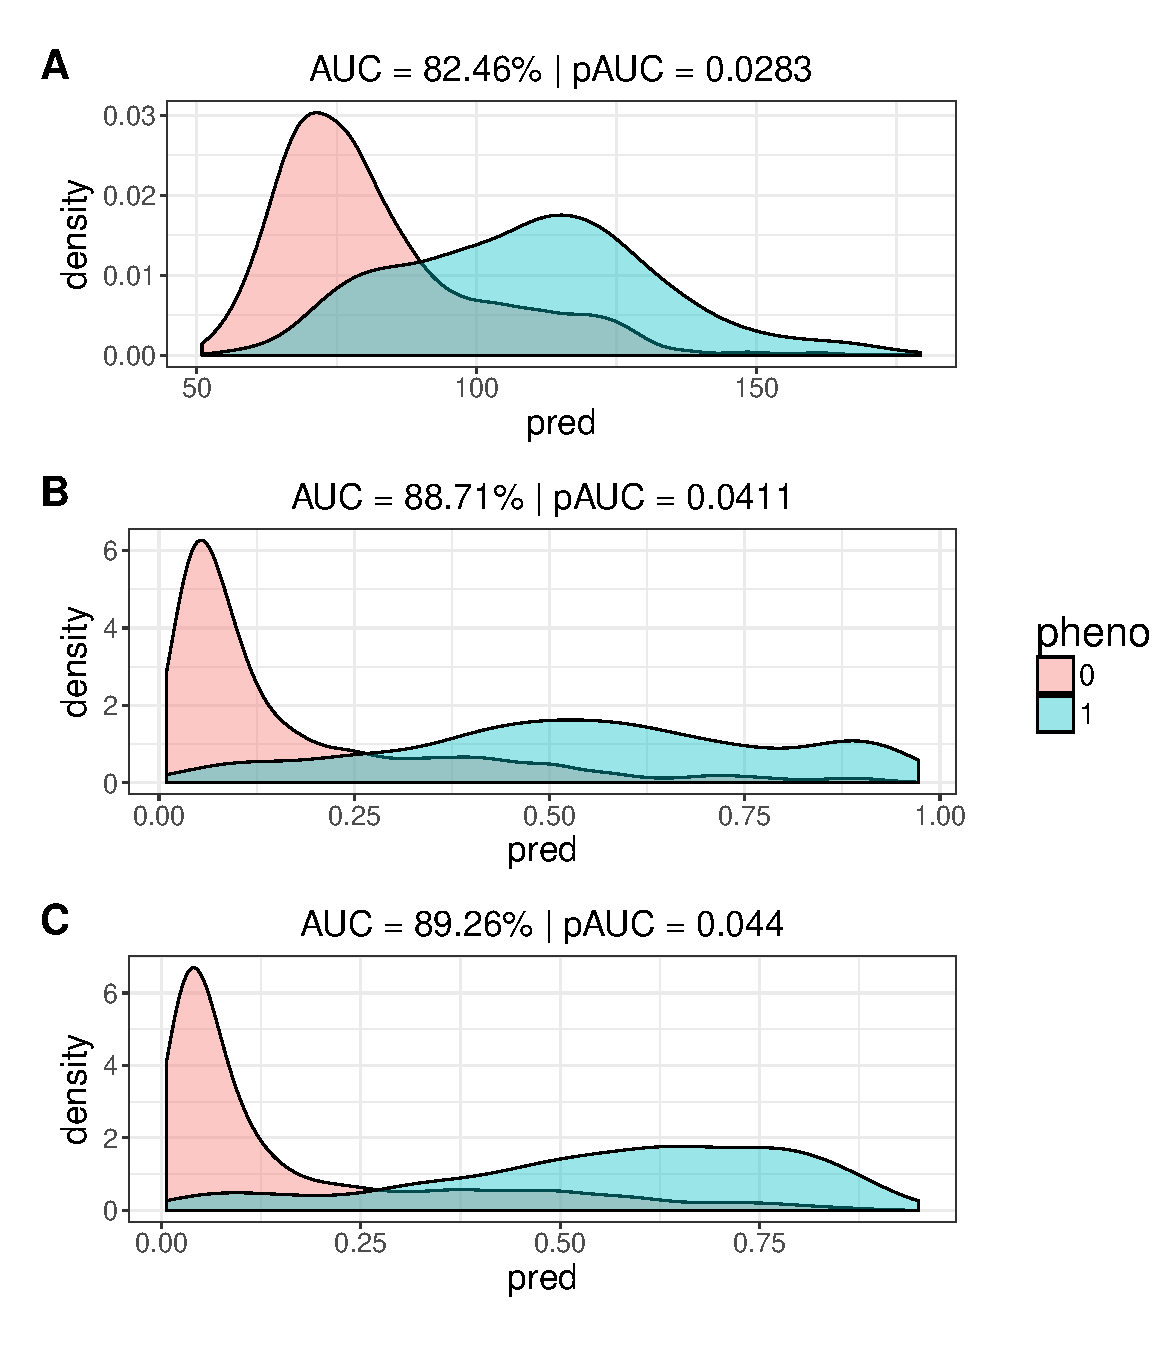
\includegraphics[width=\textwidth]{supp-score-densities}}
\caption{Density of polygenic risk scores for the ``C+T'' (A), ``logit-simple'' (B) and ``logit-triple'' (C) methods for one run on the Celiac disease, training on 12,000 individuals and projecting on the remaining 3155 individuals.\label{fig:supp-score-densities}}
\end{figure}

%%%%%%%%%%%%%%%%%%%%%%%%%%%%%%%%%%%%%%%%%%%%%%%%%%%%%%%%%%%%%%%%%%%%%%%%%%%%%%%%


\end{document}
